\documentclass[a4paper]{article}
\usepackage[utf8]{inputenc}
\usepackage[T1]{fontenc}
\usepackage{fixltx2e}
\usepackage{graphicx}
\usepackage{longtable}
\usepackage{float}
\usepackage{wrapfig}
\usepackage{rotating}
\usepackage[normalem]{ulem}
\usepackage{amsmath}
\usepackage{textcomp}
\usepackage{marvosym}
\usepackage{wasysym}
\usepackage{amssymb}
\usepackage{hyperref}
\tolerance=1000
\usepackage{minted}
\usepackage[ngerman, ]{babel}
\usepackage{berasans}
\renewcommand*\familydefault{\sfdefault}
\usepackage{geometry}
\usepackage{enumerate}
\geometry{a4paper,left=30mm,right=30mm, top=35mm, bottom=35mm}
\hypersetup{ colorlinks=true, urlcolor=blue }
\date{\today}
\title{Qt Workshop}
\hypersetup{
  pdfkeywords={},
  pdfsubject={},
  pdfcreator={Emacs 24.3.1 (Org mode 8.2.5h)}}
\begin{document}

\maketitle

\section{Einführung in QML}
\label{sec-1}
\subsection{Einleitung}
\label{sec-1-1}
Qt (gesprochen: „cute“) ist ein Cross-Platform GUI Toolkit, welches in C++ geschrieben ist. Seit Version 5.0 ist der Fokus der Entwicklung auf einer neuen Technologie namens QML, einer skripting-Sprache, mit der Qt GUIs geschrieben werden können. QML ist im Moment eine der fortschrittlichsten Technologien zur GUI-Entwicklung überhaupt.

\subsubsection{Setup}
\label{sec-1-1-1}
Am einfachsten kann man Qt installieren, indem man einen der Installer für Qt 5.2.1 von \url{http://qt-project.org} herunterlädt. Auf Linux und OSX kann statt dessen auch der jeweilige Paketmanager benutzt werden. Für Windows gibt es auf der Webseite eine lange Liste von verschiedenen Compiler-Versionen. Ich empfehle die MinGW-Version, da sie als einzige ihren eigenen Compiler im Installationspaket mitbringt. Die Visual Studio-Varianten funktionieren ebenfalls, man muss jedoch Visual Studio in der passenden Version installiert haben und das initiale Setup kann etwas schwieriger sein.

Jetzt kann der mitgelieferte Qt Creator gestartet werden. Qt Creator ist eine mächtige IDE zur Entwicklung von Qt-Anwendungen. Zuerst empfehle ich, Qt Creator auf Englisch umzustellen. Die UI-Sprache kann in \emph{Einstellungen} $\rightarrow$ \emph{Umgebung} $\rightarrow$ \emph{Allgemein} $\rightarrow$ \emph{Sprache} geändert werden.

Für heute verwenden wir ausschließlich „Qt Quick UI“ Projekte, also Projekte in reinem QML ohne C++. Um ein Qt Quick UI-Projekt zu erstellen, im Qt Creator ein neues Projekt erstellen, und „Qt Quick UI“ als Projekttyp auswählen, dann das „Qt Quick Controls 1.0“ Template verwenden.

Das Qt Quick Controls 1.0 Template erstellt ein Template zum Prototyping von klassischen Desktop-Anwendungen mit Fenstern, Buttons, Texfeldern etc.

Im Qt Creator sollte jetzt folgender Code erschienen sein:

\begin{minted}[]{js}
import QtQuick 2.1
import QtQuick.Controls 1.0
import QtQuick.Window 2.0

ApplicationWindow {
    title: qsTr("Hello World")
    width: 640
    height: 480

    menuBar: MenuBar {
        Menu {
            title: qsTr("File")
            MenuItem {
                text: qsTr("Exit")
                onTriggered: Qt.quit();
            }
        }
    }

    Button {
        text: qsTr("Hello World")
        anchors.horizontalCenter: parent.horizontalCenter
        anchors.verticalCenter: parent.verticalCenter
    }
}
\end{minted}

Dieser Code ist in QML geschrieben, der Qt Modeling Language. QML ist eine Javascript-basierte Sprache, die speziell für GUI-Design entwickelt wurde.

Der Code beginnt mit \verb~import~-Statements, welche QML \emph{Modules} laden. Das Modul \verb~QtQuick.Control~ in Version \verb~1.0~ stellt etwa die Objekte \verb~Button~ und \verb~MenuBar~ zur Verfügung.

Wenn auf ein Wort eine öffnende Klammer folgt, etwa \verb~qsTr(...)~ ist das ein Funktionsaufruf. \verb~qsTr~ ist dabei der Qt-Translation Handler, welcher Strings in andere Sprachen übersetzen kann.

Wenn auf ein groß geschriebenes Wort eine öffnende geschweifte Klammer folgt, wird ein Objekt erzeugt, etwa

\begin{minted}[]{js}
Button {
    ...
}
\end{minted}

Dieser Code erzeugt etwa einen Button. Objekte können beliebig ineinander verschachtelt sein. Objekte können außerdem ähnlich wie C++-Klassen voneinander abgeleitet werden und um eigene Funktionalität erweitert werden.

Jedes Objekt hat so genannte \emph{Properties}, welche verschiedene Eigenschaften eines Objekts kontrollieren. Wann immer auf ein Wort ein Doppelpunkt folgt, wird einer dieser Properties ein Wert zugewiesen, etwa

\begin{minted}[]{js}
width: 640
\end{minted}

Dies weist der Property namens \verb~width~ den Wert \verb~640~ zu. Jedes QML-Objekt hat ein jeweils eigenes Set an Properties. Die \verb~width~-Property etwa gibt die Breite des Objekts in Pixeln an. Properties können aber nicht nur Werte sein, sondern genauso gut Expressions, Funktionen, oder andere Objekte.

Mehr Informationen zu den einzelnen Objekten und ihren Properties kann auf der Dokumentations-Webseite erlangt werden. Eine Übersicht über alle Objekttypen und ihre Eigenschaften kann hier gefunden werden: \url{http://qt-project.org} -> \href{http://qt-project.org/doc/}{Documentation} -> \href{http://qt-project.org/doc/qt-5/qmltypes.html}{QML Types} (rechte Spalte)

Am Ende ist also aller bisher gesehener Code eine einzige große Datenstruktur.

Wenn der obige Code ausgeführt wird, sollte dies folgendes Fenster erzeugen:

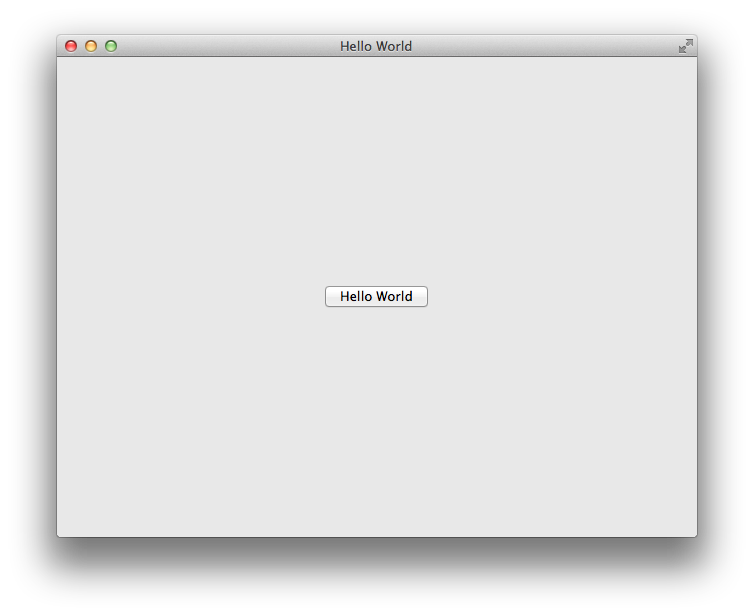
\includegraphics[width=.9\linewidth]{images/first_template_program.png}

\begin{quote}
\uline{Aufgabe:}
\begin{itemize}
\item Default-Projekt öffnen und ausführen
\item Mit Werten spielen
\item Höhe, Breite des Fensters ändern
\item Button-Text ändern
\end{itemize}
\end{quote}
\subsection{GUI-Layout}
\label{sec-1-2}
Wie bekommt man neue Controls auf ein Fenster? Prinzipiell kann jedes Control beliebig viele andere Controls enthalten. Um also einen neuen Button auf der bestehenden GUI anzuordnen, kann an beliebiger Stelle des \verb~ApplicationWindow~ ein neuer \verb~Button { ... }~ eingefügt werden. Standardmäßig befindet sich der neue Button jetzt ganz links oben in der Ecke. Die folgenden Abschnitte beschäftigen sich damit, wie diese Control nun positioniert werden kann.

\subsubsection{GUI-Designer. Tab „Design“ auf der linken Seite}
\label{sec-1-2-1}
Anders als andere GUI-Designer verändert dieser QML Designer direkt den Code! Man kann im Designer allerdings nicht alle Eigenschaften von Controls einstellen, so dass manuelle Arbeit am Code immer benötigt wird.

Der QML-Designer kennt auch nur recht wenige Control-Typen und kennt auch keine selbst erstellten Controls. Ich benutze ihn daher praktisch nie und er soll daher auch kein Fokus dieses Workshops sein.
\subsubsection{Direct Positioning}
\label{sec-1-2-2}
Alle Controls sind abgeleitet von \href{http://qt-project.org/doc/qt-5/qml-qtquick-item.html}{Item}, welches vier wichtige Properties besitzt:
\begin{itemize}
\item x, die Pixel-Position des Controls auf seinem Parent horizontal von links oben.
\item y, die Pixel-Position des Controls auf seinem Parent vertikal von links oben.
\item width, die Breite des Controls in Pixel
\item height, die Höhe des Controls in Pixel
\end{itemize}

Alle Positionierung ist dabei hierarchisch, d.h. x und y beziehen sich immer auf das Parent-Control und nicht etwa das Fenster oder den Bildschirm.

\begin{quote}
\uline{Aufgabe:}
\begin{itemize}
\item Erstellt einen Button und positioniere ihn rechts unten in der Ecke.
\item Baue einen Button auf einen Button, so dass er Platz hat.
\end{itemize}
\end{quote}
\subsubsection{Anchoring}
\label{sec-1-2-3}
Jedes Control hat eine Property Group \verb~anchors~, mit der relative Positionen zu Elter- oder Geschwister-Controls angegeben werden können. Dokumentation bei \href{http://qt-project.org/doc/qt-5/qml-qtquick-item.html}{Item}. Um Controls dabei etwa neben einem anderen Control anzuordnen, muss dieses andere Control benannt werden können. Hierzu kann jedem Control eine ID gegeben werden, über die Property \verb~id~. IDs sind jeweils global für eine Datei gebunden und sollten innerhalb einer Datei einzigartig sein.
Über die Property \verb~parent~ kann außerdem immer auf die Elter-Control zugegriffen werden.

Über die Property Group \verb~anchors~ kann nun die Control-Position relativ zu Geschwistern oder Eltern angegeben werden. Dabei kann auch lesend auf die read-only Properties \verb~top~, \verb~bottom~, \verb~left~, \verb~right~, \verb~verticalCenter~, \verb~horizontalCenter~ und \verb~baseline~ zugegriffen werden.

So können zwei Buttons etwa folgendermaßen nebeneinander positioniert werden:

\begin{minted}[]{js}
Button {
    id: b1
    text: "Button 1"
    anchors.left: parent.left
}
Button {
    id: b2
    text: "Button 2"
    anchors.left: b1.right
}
\end{minted}

\begin{quote}
\uline{Beispiel:}

Ein Button, zentriert
\begin{minted}[]{js}
Button {
    anchors.centerIn: parent
}
\end{minted}
\end{quote}

\begin{quote}
\uline{Beispiel:}

Zwei Buttons nebeneinander über die volle Breite
\begin{minted}[]{js}
Button {
    id: b1
    text: "Button 1"
    anchors.left: parent.left
    anchors.verticalCenter: parent.verticalCenter
}
Button {
    text: "Button 2"
    anchors.right: parent.right
    anchors.left: b1.right
    anchors.verticalCenter: parent.verticalCenter
}
\end{minted}
\end{quote}

Man sieht hier allerdings schon, dass die Breiten der beiden Buttons nicht gleich sind.

\begin{quote}
\uline{Beispiel:}

Zwei Buttons über die volle Breite des Fensters, gleiche Breiten:
\begin{minted}[]{js}
Button {
    text: "Button 1"
    anchors.left: parent.left
    anchors.right: parent.horizontalCenter
    anchors.verticalCenter: parent.verticalCenter
}
Button {
    text: "Button 2"
    anchors.right: parent.right
    anchors.left: parent.horizontalCenter
    anchors.verticalCenter: parent.verticalCenter
}
\end{minted}
\end{quote}

Dies wird für mehrere Buttons schnell umständlich, daher andere Lösung:

\begin{quote}
\uline{Beispiel:}

Zwei Buttons über die volle Breite des Fensters, gleiche Breiten:
\begin{minted}[]{js}
Item {
    anchors.horizontalCenter: parent.horizontalCenter
    anchors.verticalCenter: parent.verticalCenter
    Button {
        id: b1
        text: "Button 1"
    }
    Button {
        text: "Button 2"
        anchors.left: b1.right
    }
}
\end{minted}
\end{quote}

Hier werden die beiden Buttons mit einem neuen Control umschlossen, welches sich leicht zentriert positionieren lässt. Parent-Controls wachsen dabei meist dynamisch mit ihrem Inhalt, so dass das \verb~Item~ hier genau groß genug ist, um die beiden Buttons aufzunehmen.
Um zu visualisieren, was genau hier passiert kann statt eines \verb~Item~ auch ein \verb~Rectangle~ verwendet werden, welches anders als das Item eine feste Hintergrundfarbe haben kann:

\begin{minted}[]{js}
Rectangle {
    color: "red"
    anchors.centerIn: parent
    Button {
        id: b1
        text: "Button 1"
    }
    Button {
        text: "Button 2"
        anchors.left: b1.right
    }
}
\end{minted}

Im Grunde sind das alles aber nur nettere Varianten von \verb~x~, \verb~y~, \verb~width~, \verb~height~ und alle Positionierung geschieht immer noch von Hand.

\begin{quote}
\uline{Aufgabe:}
\begin{itemize}
\item Erstelle zwei Buttons nebeneinander, unten rechts in der Ecke.
\item Positioniere die beiden Buttons mit 10 Pixeln Abstand voneinander.
\end{itemize}
\end{quote}
\subsubsection{Layouts}
\label{sec-1-2-4}
Wie schon gesehen, wird es schnell umständlich, mehrere Controls gemeinsam zu positionieren. insbesondere ist es schwierig, Kontrolle über die relative Größe von Controls zueinander und im Verhältnis zur Fenstergröße zu behalten.

Die bisher verwendeten Properties werden daher meist nur für einzelne Controls eingesetzt, selten aber für mehrere Controls, die in komplexen Beziehungen zueinander stehen. Statt dessen werden hierfür Layouts verwendet. Layouts enthalten mehrere Controls und kontrollieren deren Positionierung.

So können mehrere Controls etwa mit einem \href{http://qt-project.org/doc/qt-5/qml-qtquick-layouts-rowlayout.html}{RowLayout} nebeneinander, mit einem \href{http://qt-project.org/doc/qt-5/qml-qtquick-layouts-columnlayout.html}{ColumnLayout} übereinander und mit einem \href{http://qt-project.org/doc/qt-5/qml-qtquick-layouts-gridlayout.html}{GridLayout} in einer Tabelle angeordnet werden. Dabei ist zu beachten, dass für \verb~QtQuick.Controls~ immer die genannten Layouts verwendet werden sollten. Es existieren auch noch ein Set von einfacheren Controls namens \verb~Row~, \verb~Column~ und \verb~Grid~, welche im Grunde das selbe machen, jedoch für einfachere Controls gedacht sind. So würde ein \verb~RowLayout~ etwa einen Text und einen Button so anordnen, dass deren Texte auf der selben Höhe stehen, während eine \verb~Row~ lediglich die Unterkante der Controls auf eine Höhe brächte.

Um \verb~RowLayout~, \verb~ColumnLayout~ und \verb~GridLayout~ benutzen zu können, muss \verb~QtQuick.Layouts 1.1~ importiert werden.

\begin{quote}
\uline{Beispiel:}

Zwei Buttons nebeneinander, zentriert
\begin{minted}[]{js}
RowLayout {
    anchors.centerIn: parent
    Button {
        text: "Button 1"
    }
    Button {
        text: "Button 2"
    }
}
\end{minted}
\end{quote}

Layouts sind Container-Controls, die ihre Kinder nach Regeln anordnen. Im Grunde verwende ich grundsätzlich \emph{immer} Layouts und fast nie Anchoring oder Direct Positioning.

Bei der Verwendung von Layouts ist aber zu beachten, dass Layouts volle Kontrolle über die Positionierung benötigen. Das bedeutet, dass \verb~anchors~ und \verb~x~, \verb~y~, \verb~width~ und \verb~height~ innerhalb der Kinder von Layouts nicht mehr verwendet werden dürfen.

Um dennoch erweiterte Kontrolle über die Positionierung der Controls innerhalb des Layouts zu erhalten, fügen Layouts all ihren Kindern eine \emph{attached Property} hinzu: \href{http://qt-project.org/doc/qt-5/qml-qtquick-layouts-layout.html}{Layout}.

\begin{quote}
\uline{Beispiel:}

TableView mit Plus/Minus-Button, der auto-wächst
\begin{minted}[]{js}
ColumnLayout {
    anchors.fill: parent
    TableView {
        Layout.fillHeight: true
        Layout.fillWidth: true
        TableViewColumn { title: "name" }
    }
    RowLayout {
        Button { text: "+" }
        Button { text: "-" }
    }
}
\end{minted}
\end{quote}

\begin{quote}
\uline{Aufgabe:}

Zwei Zeilen aus je: Name, Slider, SpinBox
\begin{itemize}
\item Einmal versuchen mit RowLayout und ColumnLayout
\item Einmal versuchen mit GridLayout
\end{itemize}
\end{quote}
\subsection{Properties, Signals und Slots}
\label{sec-1-3}
Mit Anchoring und Layouts lassen sich beliebige GUI-Layouts erzeugen. Die meisten GUI-Frameworks sehen hier ihre Aufgabe als beendet an und geben die Kontrolle an den Programmierer--alle weitere Funktionalität muss von Hand programmiert werden. Qt Widgets, das C++-Framework von Qt, arbeitet auch auf diese Art: Es kann mit Hilfe des Qt Designers ein GUI-Layout erzeugt werden, welches dann von der Qt Runtime erzeugt wird und mit C++-Code mit Funktionalität verknüpft wird.

Die eigentliche Innovation vom QML ist, dass GUI-Layout und Funktionalität nicht mehr von einander getrennt sind. QML kann sowohl dazu verwendet werden, Controls zu positionieren, als auch, Interaktionen zwischen Controls zu definieren. In der Praxis kann oft der größte Teil aller User-Interaktion innerhalb von QML abgehandelt werden, und nur die wenigsten Aufgaben erfordern tatsächlichen Backend-Code.

Mehr Info: \url{http://qt-project.org/doc/qt-5/qtqml-syntax-objectattributes.html}

\subsubsection{Bindings und Signal Handlers}
\label{sec-1-3-1}
Um Controls miteinander kommunizieren zu lassen, werden in Qt klassisch \emph{Signals} und \emph{Slots} verwendet. Jedes Control kann ein \emph{Signal} aussenden, etwa sendet ein Button das Signal \emph{clicked}, wenn er angeklickt wurde. Außerdem hat jedes Control \emph{Slots}, also Funktionen, die von Signals aufgerufen werden. So kann etwa ein anderer Programmteil auf das Anklicken des Buttons reagieren.

Neben solcherlei diskreter Ereignisse haben viele Controls auch veränderliche Eigenschaften, etwa den aktuellen Wert eines Sliders. Diese werden in QML als \emph{Properties} abgebildet. So haben etwa sowohl Slider als auch Spinboxes eine Property \verb~value~, die durch so genannte \emph{Bindings} miteinander verbunden werden können.

\begin{quote}
\uline{Beispiel:}

Ein Property Binding wird erstellt, indem einer Control ein Wert einer anderen Control zugewiesen wird.

\begin{minted}[]{js}
Slider {
    id: slider
}
SpinBox {
    value: slider.value
}
\end{minted}
\end{quote}

In Wirklichkeit haben wir schon mehrere dieser Property Bindings gesehen, als wir mittels \verb~anchors~ die Positionen verschiedener Controls voneinander abhängig gemacht hatten. Dabei hatten wir auch schon gesehen, dass Property Bindings nicht nur direkte eins-zu-eins-Abbildungen sein müssen, sondern auch beliebig komplexe Ausdrücke sein dürfen, etwa \verb~anchors.left: parent.left+10~.

Property Bindings sind eine gute Methode, eine Property einer Control abhängig von der Property einer anderen Control zu machen. Leider können sie nicht benutzt werden, um zwei Controls beidseitig miteinander zu synchronisieren, da dies zu einem \emph{Binding Loop} führen würde. QML erkennt Binding Loops selbstständig und bricht sie nach einigen hundert Iterationen ab. Es gibt jedoch eine elegante Umgehung dieses Problems.

Anstatt über ein direktes Binding zwei Controls miteinander zu verbinden, kann auf diskrete Property-Änderungen reagiert werden. Hierzu werden in QML so genannte \emph{Property Change Signal Handler} verwendet. Für jede Property existiert implizit immer ein Property Change Signal, welches ausgesendet wird wenn sich die Property ändert. Property Change Signals haben immer den Namen \verb~<propertyName>Changed~, also für die Property \verb~value~ etwa \verb~valueChanged~. Ein Property Change Signal Handler ist schließlich ein Slot, welcher \verb~on<propertyName>Changed~ genannt wird und immer dann aufgerufen wird, wenn das Property Change Signal ausgesendet wird.

So kann etwa ein Slider und eine SpinBox mit einem zweiseitigen Property Change Signal Handler miteinander verbunden werden, ohne dass es zu einem Binding Loop kommt.

\begin{quote}
\uline{Beispiel:}

\begin{minted}[]{js}
Slider {
    id: slider
    onValueChanged: spinbox.value = value
}
SpinBox {
    id: spinbox
    onValueChanged: slider.value = value
}
\end{minted}
\end{quote}

Property Change Signal Handler sind quasi-Funktionen, die aufgerufen werden, wann immer sich eine Property ändert.

Signal Handler existieren für jedes beliebige Signal, nicht nur Property Change Signals. So reagiert ein Button etwa auf sein Signal \verb~clicked~ in einem Signal Handler \verb~onClicked~.

\begin{quote}
\uline{Beispiel:}

Der folgende Button etwa gibt \verb~"Hello, World!"~ aus, wenn er angeklickt wird:
\begin{minted}[]{js}
Button {
    text: "Click Me!"
    width: 200
    onClicked: print("Hello, World!")
}
\end{minted}
\end{quote}

Signal Handler sind auch nicht auf einzelne Zeilen beschränkt, sondern können beliebig komplex sein. Wenn ein Signal Handler mehr als eine Zeile umfasst, muss er von geschweiften Klammern umschlossen werden.

\begin{quote}
\uline{Beispiel:}

Der folgende Button ändert seine Breite jedes mal wenn er angeklickt wird:

\begin{minted}[]{js}
Button {
    text: "Click Me!"
    width: 200
    onClicked: {
        if (width === 200) {
            width = 400
        } else {
            width = 200
        }
    }
}
\end{minted}
\end{quote}

Solcherlei binäre Entscheidungen sind in GUIs recht häufig. Es wird in diesen Fällen daher gern der Ternäre Operator benutzt. Das obige Beispiel ließe sich damit etwa folgendermaßen ausdrücken: \verb~onClicked: width = width==200 ? 400 : 200~. Dieses Muster kann auch an anderen Stellen eingesetzt werden, etwa \verb~text: width==200 ? "narrow" : "wide"~.

Spinboxen reagieren by default auf jede Eingabe sofort. Wird etwa die Zahl \verb~10~ eingegeben, so springt der Wert erst auf \verb~1~, dann auf \verb~10~. Dies kann mitunter problematisch sein. Es ist bei Spinboxen daher oft sinnvoll, nicht auf \verb~onValueChanged~, sondern auf \verb~onEditingFinished~ zu reagieren.

Ein weiteres interessantes Signal ist \verb~Control.completed~, welches von der attached Property \verb~Control~ ausgesendet wird, wenn ein Control fertig initialisiert wurde. Der entsprechende Signal Handler heißt \verb~Control.onCompleted~. Es ist manchmal wichtig, einige Properties erst zu manipulieren, wenn ein Control vollständig aufgebaut wurde.

\begin{quote}
\uline{Aufgabe:}

Erforsche mit Hilfe von \verb~Component.onCompleted~ die Initialisierungsreihenfolge eines Programmes. Wie ändert sich die Reihenfolge, wenn Layouts im Programm vorkommen?
\end{quote}
\subsubsection{Eine Control selber bauen}
\label{sec-1-3-2}
Eine große Stärke von QML ist es, dass es sehr einfach ist, eigene Controls zu bauen. Im Folgenden wollen wir zwei Controls selbst definieren, einen Button und einen Slider.

Hier werden wir zum ersten Mal nicht mehr mit \verb~QtQuick.Controls~ arbeiten, sondern mit reinem \verb~QtQuick 2.2~. \verb~QtQuick.Controls~ enthält die üblichen Controls für WIMP-Interfaces, wie man sie auf den Desktop-Plattformen kennt. Die Controls in \verb~QtQuick~ sind jedoch einfach genug, dass sie auf allen Plattformen des Qt-Frameworks unterstützt werden, also unter anderem Windows, OSX, Linux, Android und iOS.

\begin{quote}
\uline{Beispiel:}

Eine der einfachsten möglichen Controls ist sicher ein Button. Im Grunde ist ein Button nichts anderes als ein Rechteck mit Text darauf, welches sich anklicken lässt. In QML ausgedrückt also ein \verb~Rectangle~ mit einem \verb~Text~ und einer \verb~MouseArea~.

\begin{minted}[]{js}
import QtQuick 2.2

Rectangle {
    id: root
    implicitWidth: 108
    implicitHeight: 26
    color: mousearea.pressed ? 'lightgrey' : 'darkgrey'
    Text {
        anchors.centerIn: parent
        text: "Click Me!"
    }
    MouseArea {
        id: mousearea
        anchors.fill: parent
    }
}
\end{minted}

Ähnlich wie ein echter Button sollte dieser Button nun auch seinen Text als Property setzbar machen. Man kann in QML sehr leicht an jeder Stelle eine Property definieren:

\begin{minted}[]{js}
Rectangle {
    property string text: "Click Me!"
    // ...
    Text {
        anchors.centerIn: parent
        text: parent.text
    }
}
\end{minted}

So bekommt das Rectangle eine neue Property vom Typ \verb~string~ mit Namen \verb~text~, welche vom Text-Control dann übernommen wird.

Neben der Property \verb~text~ hat ein echter Button auch eine Property \verb~pressed~, welche angibt ob der Button gerade gedrückt wird oder nicht. Auch das lässt sich leicht implementieren.

\begin{minted}[]{js}
Rectangle {
    property alias pressed: mousearea.pressed
    // ...
    MouseArea {
        id: mousearea
        anchors.fill: parent
    }
}
\end{minted}

Eine Property vom Typ \verb~alias~ ist keine echte eigenständige Property, sondern lediglich ein alternativer Name, um auf die originale Property zuzugreifen. Somit lässt sich auch die Farbzuweisung etwas erleichtern: \verb~color: pressed ? 'lightgrey' : 'darkgrey'~.

Außerdem hat ein echter Button noch ein Signal \verb~clicked~, welches ausgesendet wird wenn der Button gedrückt wird. Auch Dieses lässt sich aus der MouseArea übernehmen:

\begin{minted}[]{js}
Rectangle {
    signal clicked
    // ...
    MouseArea {
        // ...
        onClicked: parent.clicked()
    }
}
\end{minted}

Schließlich hat ein echter Button noch keine statische Größe, sondern passt sich der Größe seines Inhaltes an. Hierfür kann man sich der Property \verb~contentWidth~ des Textes bedienen:

\begin{minted}[]{js}
import QtQuick 2.1

Rectangle {
    id: root
    width: text.contentWidth + 10
    height: text.contentHeight + 10
    color: mousearea.pressed? 'lightgrey' : 'darkgrey'

    signal clicked
    property string text: "Click Me!"

    Text {
        id: text
        anchors.centerIn: parent
        text: parent.text
    }
    MouseArea {
        anchors.fill: parent
        onClicked: root.clicked()
    }
}
\end{minted}
\end{quote}

\begin{quote}
\uline{Beispiel:}

Eine etwas kompliziertere Control ist ein Slider, mit Property \verb~value~, \verb~minimumValue~ und \verb~maximumValue~, und eigenen Grafiken.

Anstatt wie beim Button lediglich Rechtecke zu benutzen, sollten diesmal Grafiken verwendet werden. Dafür habe ich zwei (wunderschöne) Grafiken vorbereitet, eine für das Slider-Handle und eine für den Hintergrund.


\includegraphics[width=24px]{images/groove.png}
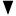
\includegraphics[width=16px]{images/handle.png}

Um Grafiken zu zeichnen, werden in QML Image Controls benutzt. Da das Control selbst höher ist als die Groove und breiter als das Handle, muss es als eigenes Control gebaut werden. Ein einfaches, durchsichtiges Control ist das Item.

\begin{minted}[]{js}
Item {
    width: 100
    height: 24
    Image {
        id: groove
        source: 'groove.png'
        height: 16
        width: parent.width
        anchors.verticalCenter: parent.verticalCenter
    }
    Image {
        id: handle
        source: 'handle.png'
        anchors.top: parent.top
        anchors.bottom: parent.bottom
    }
}
\end{minted}

Dies funktioniert für das Handle gut, verzerrt jedoch den Groove sehr stark in die Breite. Statt dessen kann eine spezielle Art Image verwendet werden, welche sich an die Größe der Control anpassen kann, das BorderImage. Ein BorderImage besteht aus neun Quadranten, wobei die Ecken jeweils in den Ecken des Controls gezeichnet werden und die Seiten entsprechend der Control-Größe verlängert werden.

\begin{minted}[]{js}
Item {
    width: 100
    height: 24
    BorderImage {
        id: groove
        source: 'groove.png'
        border { left: 8; right: 8; top:8; bottom: 8 }
        height: 16
        width: parent.width
        anchors.verticalCenter: parent.verticalCenter
    }
    Image {
        id: handle
        source: 'handle.png'
        anchors.top: parent.top
        anchors.bottom: parent.bottom
    }
}
\end{minted}

Nun fehlt nur noch die Maus-Interaktion, um das Handle zu verschieben. Hierfür bietet die MouseArea eine spezielle Property Group \verb~drag~, die sich um Verschiebung kümmert:

\begin{minted}[]{js}
MouseArea {
    anchors.fill: parent
    drag.target: handle
    drag.axis: Drag.XAxis
    drag.minimumX: 0
    drag.maximumX: groove.width-handle.width
}
\end{minted}

Als nächstes sollte sich das Handle auch bewegen, wenn man an beliebige Stelle in den Groove klickt. Hierfür kann der \verb~onClicked~ Signal Handler der MouseArea verwendet werden. Das Signal \verb~clicked~ stellt hierbei Informationen über den Klick, wie etwa die Position des Klicks, über die Variable \verb~mouse~ zur Verfügung. Entsprechend kann diese Information auch im \verb~onClicked~ Signal Handler abgerufen werden.

\begin{minted}[]{js}
onClicked: {
    if (mouse.x < handle.width/2) {
        handle.x = 0
    } else if (mouse.x > groove.width-handle.width/2) {
        handle.x = groove.width-handle.width
    } else {
        handle.x = mouse.x - handle.width/2
    }
}
\end{minted}

Wie auch der echte Slider sollte auch unser Slider drei Properties \verb~value~, \verb~minimumValue~ und \verb~maximumValue~ besitzen, die sich automatisch updaten wenn das Handle bewegt wird bzw automatisch das Handle bewegen, wenn die Property geändert wird.

Da sich die Position des Handles sowohl durch Klicken auf den Groove als auch durch Draggen des Handles verändern kann, muss die Logik zum Umrechnen der Handle-Position zu \verb~value~ an zwei Stellen geschehen. Um sich diese Duplikation von Arbeit abzunehmen, kann eine Javascript-Funktion implementiert werden.

\begin{minted}[]{js}
Item {
    width: 108
    height: 26
    anchors.centerIn: parent

    property real value: 0
    property real minimumValue: 0
    property real maximumValue: 100
    onValueChanged: {
        handle.x = (value-minimumValue) / (maximumValue-minimumValue)
                   * (width-handle.width)
    }

    BorderImage {
        id: groove
        source: 'groove.png'
        border { left:8; right: 8; top:8; bottom: 8 }
        height: 16
        width: parent.width
        anchors.verticalCenter: parent.verticalCenter
    }
    Image {
        id: handle
        source: 'handle.png'
        width: height
        anchors.top: parent.top
        anchors.bottom: parent.bottom
    }
    MouseArea {
        anchors.fill: parent
        drag.target: handle
        drag.axis: Drag.XAxis
        drag.minimumX: 0
        drag.maximumX: groove.width-handle.width
        function updateValue() {
            parent.value = handle.x/(groove.width-handle.width) *
                   (parent.maximumValue-parent.minimumValue) +
                   parent.minimumValue
        }
        onClicked: {
            if (mouse.x < handle.width/2) {
                handle.x = 0
            } else if (mouse.x > groove.width-handle.width/2) {
                handle.x = groove.width-handle.width
            } else {
                handle.x = mouse.x - handle.width/2
            }
            updateValue()
        }
        onPositionChanged: updateValue()
    }
}
\end{minted}
\end{quote}

\begin{quote}
\uline{Aufgabe:}

Die MouseArea bietet außerdem ein Signal \verb~onWheel~. Baue den Slider so um, dass er auf Scroll-Events reagiert.
\end{quote}
\subsection{Components und Modules}
\label{sec-1-4}
Nun wäre es schön, diese Controls so abspeichern zu können, dass sie ähnlich wie ein Slider oder Button direkt im QML verwendet werden können ohne den gesamten Quellcode jedes mal einfügen zu müssen. Controls sind in QML einfach nur erreichbare Dateien. Um unsere beiden Controls als wiederverwendbare Controls abzuspeichern, muss man sie lediglich als Datei speichern. Die Controls sind dann unter ihrem Dateinamen erreichbar.

Speichert man also den selbst gebauten Button als \emph{MyButton.qml} und den selbst gebauten Slider als \emph{MySlider.qml}, kann man sie einfach als \verb~MyButton { ... }~ bzw. \verb~MySlider { ... }~ verwenden. dabei sind alle Top-Level Properties nach außen hin sichtbar. IDs gelten allerdings immer nur innerhalb einer Datei und sind von außen nicht erreichbar.

Hat man nun einige Controls gebaut, kann man sie auch als Modul verpacken, so dass wir etwa all unsere selbst gebauten Controls per \verb~import MyControls 0.1~ erreichbar machen können.

Modules sind schlicht Ordner, die Controls und eine Datei \verb~qmldir~ enthalten. \verb~qmldir~ ist eine einfache Textdatei, die das Modul benennt und alle Controls auflistet:

\begin{verbatim}
module MyComponents
MyButton 1.0 MyButton.qml
MySlider 1.0 MySlider.qml
\end{verbatim}

Speichert man diese Datei und die beiden Controls in einem Ordner \emph{MyControls}, so kann dieser als Modul verwendet werden.

Damit Qt Creator diese Module allerdings finden kann, muss in der Projektdatei die Variable \verb~importPaths: [ "path/to/modules" ]~ setzen. Im Regelfall wird dies \verb~importPaths: [ "." ]~ sein.

\begin{quote}
\uline{Aufgabe:}

Schreibe ein neues Control, welches einen Namen, einen Slider und eine Spinbox beinhaltet und einen Namen und einen Wert auf zwei gemeinsamen Properties exposed.
\end{quote}
\section{Integration von QML und C++}
\label{sec-2}
\subsection{Technology Overview}
\label{sec-2-1}
Ein kurzer Abriss der Vergangenheit von Qt
\begin{itemize}
\item Qt ist ein Framework zum Application Development, nicht nur für grafische GUIs.
\item Qt wurde 1991 von Trolltech entwickelt, dann an Nokia und schließlich Digia verkauft.
\item Qt ist GPL, LGPL und kommerziell lizenziert, kann also kostenlos benutzt werden solange man dynamisch linkt, oder kostenpflichtig, wenn man statisch linken muss.
\item Qt wird unter anderem für Skype, VirtualBox, VLC, Google Earth und ELSTER verwendet.
\item Bis vor wenigen Jahren war Qt ein reines C++ Framework, seit 4.3 auch mit Skripting-Umgebung, die schließlich mit Qt 5.0 in QML resultierte.
\end{itemize}

Wir kennen bereits QML. QML ist eine Programmiersprache basierend auf Javascript, mit Objekten aus der Library Qt Quick:
\begin{itemize}
\item Qt Quick und Qt Quick Controls sind Module, die teils in QML, teils in C++ implementiert sind.
\item Wir haben schon gesehen, Qt Quick sind Basiscontrols wie Rechtecke und MouseAreas (gut für Smartphones), Qt Quick Controls sind High-level Controls wie Buttons und Listen (nur für Desktop).
\end{itemize}

Die C++ Klassen in Qt sind in verschiedene Module kategorisiert:
\begin{itemize}
\item Qt Core (Threading, Resource Handling, QString, State Machines, Internationalization\ldots{})
\item Qt GUI (Window, OpenGL, Images, Painting\ldots{})
\item Qt Widgets (Damit hat man früher GUIs entwickelt, UI-Files)
\item Qt Networking
\item Qt Multimedia (soweit ich sehen kann keine Blockverarbeitung--Die Welt braucht ein neues portaudio)
\item Qt QML (QML-Dateien laden, QML-Objekte erzeugen, mit QML interagieren)
\end{itemize}

Die Qt-Bibliotheken implementieren in C++ eine eigene Standardbibliothek. Viele Leute sagen, Qt macht C++ benutzbar. Qt ist außerdem eine sehr moderne Bibliothek, mit C++11 Unterstützung, modernen Iteratoren, Lambdas und mächtigen Collection-Klassen.

Heute soll es um zwei Dinge gehen:
\begin{itemize}
\item Ein Kochrezept, wie man ein Qt/QML-Programm deployt.
\item Einige Beispiele, wie man Qt/C++ und QML verbinden kann.
\end{itemize}
\subsection{C++ Host Applications}
\label{sec-2-2}
Bisher haben wir ein Programm namens \verb~qmlscene~ verwendet, um QML-Dateien als Programme auszuführen. Heute wollen wir sehen, wie wir QML mit C++ verbinden können und eigenständige Anwendungen entwickeln können. Dazu müssen wir ein Host-Programm in C++ schreiben, welches den QML-Code ausführt und ihn mit dem C++-Code verbindet.

Dafür öffnen wir zuerst ein Template-Projekt. Im Qt Creator, erstelle ein neues Projekt vom Typ „Qt Quick Application“ und wähle dann das Template „Qt Quick Controls 1.0“.

Das Template erzeugt im Grunde drei Dateien:
\begin{itemize}
\item \emph{main.qml}, unser QML-Code (wie gehabt)
\item \emph{main.cpp}, unsere Host-Application, die den QML-Code lädt
\item \emph{*.pro}, die Projektdatei
\end{itemize}

Dies erzeugt ein Projekt mit einer C++-Basisklasse, in die wir unseren eigenen Code einbetten können sowie einem plattformunabhängigen Backend, welches den QML-Code lädt und für alle unterstützten Plattformen ein funktionstüchtiges Binary erzeugt.

Leider wird hier eine Projektstruktur verwendet, die für Android, iPhone und Desktop gleichermaßen funktionieren muss. Dabei wird aber einiges an Lesbarkeit und Verständlichkeit geopfert. Statt dessen möchte ich eine minimale Struktur vorstellen, die gerade ausreicht um auf Desktop zu laufen.

\begin{itemize}
\item In Qt Creator, erstelle ein neues Projekt, diesmal vom Typ „Other Projects“ $\rightarrow$ „Empty Qt Project“
Dies erzeugt eine leere Projektdatei. In der Projektdatei fügen wir folgenden Code ein, um ein minimales Set an Libraries für ein gemischtes C++/QML Projekt zu laden:

\begin{verbatim}
QT          += core qml
TARGET       = Minimal
TEMPLATE     = app
\end{verbatim}

Dies kompiliert das Projekt mit dem Namen \verb~Minimal~ als Desktop-Anwendung (\verb~app~) mit den Libraries \emph{QtCore} und \emph{QtQml}.

\item Nun fügen wir eine C++-Quelldatei hinzu. Dazu Rechtsklick auf das Projekt, „Add New\ldots{}“ $\rightarrow$ „C++ Source File“ mit Dateiname \emph{main.cpp}

\begin{minted}[]{cpp}
#include <QGuiApplication>
#include <QQmlApplicationEngine>
#include <QWindow>
#include <QDebug>

int main(int argc, char *argv[])
{
    QGuiApplication app(argc, argv);
    QQmlApplicationEngine engine("main.qml");
    if (engine.rootObjects().length() > 0) {
        QWindow *mainWindow = (QWindow*)engine.rootObjects()[0];
        mainWindow->setVisible(true);
    }
    return app.exec();
}
\end{minted}

Dies ist eine minimale Anwendung, die eine \verb~QGuiApplication~ und eine \verb~QQmlApplicationEngine~ startet, eine QML-Datei lädt und das Programm ausführt.

\item Jetzt fehlt nur noch eine QML-Datei. Wieder Rechtsklick auf das Projekt, „Add New\ldots{}“ $\rightarrow$ „QML File (Qt Quick 2)“ mit Dateiname \emph{main.qml}:

\begin{minted}[]{js}
import QtQuick.Controls 1.1
ApplicationWindow {}
\end{minted}

\item Bevor wir das Projekt nun bauen, empfehle ich, links in der Liste auf „Projects“ klicken und „Shadow Build“ ausschalten. So wird die Binary nicht in einem Ordner parallel zum Projektordner gebaut, sondern im Ordner „release“ und „debug“ innerhalb des Projektverzeichnisses.
\item Auf dem Mac ist das Resultat der Kompilierung keine \emph{*.exe}, sondern ein App Bundle, in welches die QML-Dateien kopiert werden müssen, damit sie von der Binary gefunden werden. Dies kann in der Projektdatei über folgenden Befehl realisiert werden:
\begin{verbatim}
macx {
    QmlFiles.path = Contents/MacOS
    QmlFiles.files = $$files(*.qml)
    QMAKE_BUNDLE_DATA += QmlFiles
}
\end{verbatim}
Die Auszeichnung über \verb~macx { ... }~ sorgt dabei dafür, dass diese Anweisungen auf anderen Plattformen nicht ausgeführt werden.
\end{itemize}

\begin{quote}
\textbf{Warnung:}

QML Project Files (\emph{*.qmlproject}), wie wir sie von gestern von QML-Projekten kennen, sind einfach zu schreiben und zu verstehen. QMake project files (\emph{*.pro}), wie wir sie heute verwenden, sind schrecklich komplex, mächtig und schwierig. Falls irgendwie möglich, sollten wir versuchen, die Finger von ihnen zu lassen und uns aufs Wesentlichste zu konzentrieren.

Doku: \href{http://qt-project.org/doc/qt-4.8/qmake-project-files.html}{QMake Project Files} \href{http://qt-project.org/doc/qt-5/qmake-advanced-usage.html}{QMake Advanced Usage} \href{http://qt-project.org/doc/qt-5/qmake-variable-reference.html}{QMake Variable Reference}
\end{quote}

\begin{quote}
\uline{Aufgabe:}

Portiert das gestrige Projekt auf die selbst gebaute \verb~exe~. Damit das Modul \verb~MyComponents~ geladen werden kann, muss es in den debug/release-Ordner kopiert werden. Im Zweifel kann ein eigener QML-Import-Path mit der Funktion \verb~QQmlEngine::addImportPath~ und ein eigener QML-Plugin-Path mit \verb~QQmlEngine::addPluginPath~ hinzugefügt werden.
\end{quote}
\subsection{Deployment}
\label{sec-2-3}
Das Ziel ist es nun, ein QML-Programm als self-Contained Executable auszuliefern, welches nicht mehr auf \verb~qmlscene~ oder einer bestehenden Qt-Installation basiert. Es gibt einige Anleitungen und fiese Tricks, dies im QMake Project File zu implementieren, ich habe aber noch keine verständliche und allgemeingültige Lösung gefunden.

Die hier vorgestellte Lösung ist nicht elegant oder automatisiert, aber schnell und effektiv.

Zuerst müssen alle Ressourcen, also Bilder, QML-Dateien und Libraries in den Release-Ordner kopiert werden. Dann müssen noch genau die benötigten DLLs aus der Qt-Installation dazu gelegt werden, damit die Executable ausgeführt werden kann. Es ist weder einfach noch offensichtlich, welche der Libraries benötigt werden und welche nicht. Grundsätzlich sind alle Libraries jeweils in zwei Versionen vorhanden: Release-Libraries und auf \emph{*d.dll} endende Debug-Libraries.

Hier ist ein einfacher Trick, mit dem auf Windows der richtige Satz an Libraries gefunden werden kann:
\begin{itemize}
\item Alle DLLs aus \verb~C:\Qt\5.2.1\mingw48_32\bin~ in den Release-Ordner kopieren.
\item Das Programm per Doppelklick ausführen.
\item Während das Programm läuft, alle DLLs löschen und alle in Benutzung befindlichen überspringen.
Das ist nicht die feine englische Art, aber das funktioniert.
\end{itemize}
\subsection{Application Icon}
\label{sec-2-4}
Um einer Anwendung ein professionelles Gesicht zu geben, sollte die Anwendung ein Icon bekommen. Hier zeigt sich die Stärke von Qt zur Anwendungsentwicklung: Einfache Dinge sind einfach:
\begin{minted}[]{cpp}
mainWindow->setIcon(QIcon("icon.png"));
\end{minted}
\subsection{Lokalisation}
\label{sec-2-5}
Qt bietet ein \href{http://qt-project.org/doc/qt-5/linguist-programmers.html}{mächtiges Lokalisations-System}, mit dem sich eine Anwendung abhängig von der Systemsprache in verschiedene Sprachen übersetzen lässt.

In QML müssen dafür alle Strings mit dem Qt Translation Handler \verb~qsTr( ... )~ umschlossen werden. In Qt heißt gibt es diese Funktion ebenfalls als \verb~tr( ... )~.

Das Übersetzungssystem von Qt scannt nun die Projektdatei und sucht nach übersetzbaren Dateien. Das System weiß von Haus aus bereits von allen C++-Quelldateien des Projekts, kennt aber leider die QML-Sourcen nicht, da sie nicht Teil der zu kompilierenden Quellen innerhalb der Projektdatei sind sondern zur Laufzeit geladen werden.

Um die QML-Quellen dennoch als zu übersetzende Quellen zu registrieren, müssen folgende Anweisungen in die Projektdatei eingefügt werden:

\begin{verbatim}
TRANSLATIONS += german.ts
lupdate_only {
    SOURCES += *.qml
}
\end{verbatim}

Die erste Zeile deklariert den Namen der Übersetzungesdatei, die zweite Anweisung registriert QML-Dateien für \verb~lupdate~, das Qt-Übersetzungesprogramm.

Nun kann unter Tools $\rightarrow$ External $\rightarrow$ Linguist $\rightarrow$ Update Translation die \verb~*.ts~-Datei erstellt werden. Je nach Windows-Version kann \verb~lupdate.exe~ nur als Admin ausgeführt werden, da es „update“ im Dateinamen enthält. In diesem Fall muss \verb~lupdate.exe~ umbenannt werden und es in den Qt-Creator-Einstellungen entsprechend registriert werden. Dies kann unter Tools $\rightarrow$ External $\rightarrow$ Configure eingestellt werden.

Die von \verb~lupdate~ neu erstellte Datei \verb~application_de.ts~ kann nun mit dem bei Qt mitgelieferten Programm Qt Linguist geöffnet werden. In Qt Linguist können Übersetzungen für die einzelnen Strings des Programms in der \verb~*.ts~-Datei eingetragen werden.

Unter Tools $\rightarrow$ External $\rightarrow$ Linguist $\rightarrow$ Release Translation kann nun die fertig übersetzte \verb~*.ts~-Datei in eine ladbare, komprimierte \verb~*.qm~-Datei kompiliert werden.

In \emph{main.cpp} kann nun \textbf{vor} dem Starten der \verb~QQmlEngine~ Code eingefügt werden, der die Übersetzung lädt:
\begin{minted}[]{cpp}
QTranslator translator;
translator.load("german");
app.installTranslator(&translator);
\end{minted}

Es können auf diese Art beliebig viele Übersetzungen geladen werden. Angezeigt wird immer die passende Systemsprache.
\subsection{Auslagerung der Dateien in Ressourcen}
\label{sec-2-6}
Im Moment werden noch alle Ressourcen wie Bilder oder QML-Dateien als unveränderte Quelldateien ausgeliefert. In vielen Situationen kann es nützlich sein, diese Dateien in die Anwendung einbetten zu wollen und sie so zu verstecken. Qt bietet einen Mechanismus, um \href{http://qt-project.org/doc/qt-5.0/qtcore/resources.html}{beliebige Ressourcen in die Anwendung einzukompilieren}:

Hierfür muss in Qt Creator eine neue Resource-Datei erstellt werden, und dann die gewünschten Dateien mit beliebigen Präfixen einbinden. Resource-Dateien sind eigentlich nicht eigenständige Dateien, sondern lediglich Dateilisten, die in die Anwendung mit einkompiliert werden. Es ist daher auch oft einfacher, nicht die Qt Creator GUI zum Einbinden zu verwenden, sondern die Resource-Datei von Hand in einem Texteditor zu öffnen und Dateien dort selbst einzutragen.

Um nun im laufenden Programm auf Dateien aus den Ressourcen zuzugreifen, müssen lediglich ihre Pfade geändert werden:
\begin{itemize}
\item Alle String-Pfade auf \verb~qrc:///prefix/file~ ändern.
\item Alle Url-Pfade auf \verb~:/prefix/file~ ändern.
\end{itemize}

Theoretisch sollten diese beiden Schreibweisen austauschbar sein. Leider ist dem nicht so und ich konnte keine Dokumentation finden, wann welche Schreibweise erforderlich ist.
\begin{itemize}
\item \verb~QQmlApplicationEngine~ benötigt eine \verb~QUrl~ anstatt eines Strings, um auf Ressourcen zuzugreifen.
\item Um Module einzubinden, muss zuerst mittels \verb~QQmlEngine::addImportPath~ ein Import Path in die Ressourcen gesetzt werden. Damit können auch Module eingebunden werden. Allerdings müssen dort auch in der \verb~qmldir~-Datei die Pfade gegebenenfalls in \verb~qrc://~-Pfade umgeschrieben werden.
\end{itemize}
\subsection{Intermission}
\label{sec-2-7}
An dieser Stelle sollten wir einen Moment innehalten: Wir haben jetzt eine vollständige Anwendung mit Qt und QML gebaut. Eine reine, deploybare Binärdatei, komplett mit Programmicon, einkomplierten Ressourcen und Übersetzung. Und all das, in 20 Zeilen C++!.

Dieser selbe Code kann auch von einer Library aus gestartet werden, um von einem beliebigen Programm aus eine Qt-Anwendung zu starten! Und so fummelig das auch war, all unsere GUI-Logik ist davon völlig unberührt geblieben!

Nun zum zweiten Teil dieses Kapitels: Echte Interaktion zwischen QML und C++.
\subsection{Interaktion von QML und C++}
\label{sec-2-8}
Es gibt zwei Methoden, QML mit C++ sprechen zu lassen: Als Teil der Host-Anwendung oder als separat geladenes Plugin. Ein Plugin zu schreiben ist oft ein klein wenig mehr Aufwand, lohnt sich aber, da ein wohldefiniertes und debuggtes Plugin sehr viel leichter zu maintainen ist als ein großer Wust an Klassen, die in der Host-Anwendung registriert werden.

Die Idee ist immer, bestehende Qt-Klassen abzuleiten und \href{http://qt-project.org/doc/qt-5/properties.html}{in QML zu registrieren}:
Um eine Klasse Qt-Konform zu schreiben, müssen folgende Randbedingungen eingehalten werden:
\begin{itemize}
\item Die Klasse muss von \href{http://qt-project.org/doc/qt-5/qobject.html}{QObject} oder einer anderen Qt-Klasse abgeleitet sein.
\item Die Klasse muss das Makro \verb~Q_OBJECT~ enthalten, um sie als QObject auszuzeichnen.
\item Die Klasse kann \verb~signals~, \verb~slots~ und \verb~Q_PROPERTY~ enthalten.
\item Die Klasse muss Wertänderungen seiner Properties mit Hilfe von \verb~emit signal~ kennzeichnen.
\item \verb~qDebug()~ kann als Ausgabe benutzt werden. (vorher \verb~#include <QDebug>~)
\end{itemize}

Eine einfache C++-Klasse könnte etwa folgendermaßen aussehen:

\begin{quote}
\uline{Beispiel:}

\begin{minted}[]{cpp}
class Counter : public QObject {
    Q_OBJECT
    Q_PROPERTY(int value READ value WRITE setValue NOTIFY valueChanged)

public:
    Counter();
    ~Counter();

    int value();

public slots:
    void setValue(int value);
    void increment();

signals:
    void valueChanged(int value);

private:
    int m_value;
};

// In main():
#include <QtQml>
qmlRegisterType<Counter>("Backend", 1, 0, "Counter");
\end{minted}
\end{quote}

Diese Klasse kann nun in QML mittels \verb~import Backend 1.0~ eingebunden werden und als \verb~Counter~ benutzt werden. Man könnte nun einen Button bauen, welcher den Counter incremented und eine Textanzeige, welche den aktuellen Wert des Counters ausgibt. \verb~value~ kann dabei als Property wie jede andere QML-Property genutzt werden.

Als Randnotiz: Für formatiertes Ausgeben von Text, kann in QML und Qt die String-Funktion \verb~arg()~ verwendet werden, welche String-Ersetzung von Platzhaltern wie \verb~"%1"~ durchführt. \verb~arg()~ ersetzt jeweils nur den niedrigsten Platzhalter, kann aber mehrmals aufgerufen werden, etwa \verb~"%1, %2!".arg("Hello").arg("World")~.

\begin{quote}
\uline{Aufgabe:}

Schreibe eine C++-Klasse, die den Wert eines Sliders mitverfolgt und in C++ ausgibt. In einem echten Programm könnte man diesen Wert etwa auf die Festplatte speichern oder über ein Netzwerk übertragen wollen.
\end{quote}

Dieser Code wird im Moment noch in \verb~main()~ in die Host-Anwendung eingebettet. Um den selben Code als dynamisch ladbares Plugin zu kompilieren, muss ein neues Projekt vom Typ „Qt Quick 2 Extension Plugin“ erstellt werden.

Im Projekt-Wizard nun als Klassenname „Counter“
qt angeben und in \emph{counter.h} bzw. \emph{counter.cpp} den bestehenden Code einsetzen. Gegebenenfalls kann noch in den Dateien \emph{*plugin} die URI oder bei \verb~qmlRegisterType~ der Klassenname geändert werden.

Wird dieses Projekt kompiliert, kann die erstellte Library sowie die \verb~qmldir~-Datei wie bei QML-Modules in einen passenden Ordner kopiert werden und von QML aus mit \verb~import ModulName 1.0~ geladen werden.

Plugins können auch problemlos von \verb~qmlscene~-Projekten geladen werden--es muss allerdings immer auf die korrekte Kompilationsart geachtet werden: Debug/Release und 32/64-Bit müssen in Plugin und Anwendung identisch sein.

\begin{quote}
\uline{Aufgabe:}

Baut eure eigene Klasse einmal in die Host-Anwendung und einmal als Plugin.
\end{quote}

\begin{quote}
\uline{Beispiel:}

Eine C++-Klasse/QML-Plugin, die die aktuelle Uhrzeit als Properties darstellt. In QML kann damit einfach eine Zeit-Anzeige gebaut werden.

Dazu kann die Klasse \verb~QDateTime~ verwendet werden, welche den statischen Member \verb~currentDateTime()~ besitzt. \verb~QDateTime~ gibt die aktuelle Uhrzeit als \verb~QTime~ über die Funktion \verb~time()~ aus. Neben \verb~QDateTime~ gibt es auch noch \verb~QTime~. \verb~QTime~ ist \verb~QDateTime~ sehr ähnlich, hat jedoch keine Kenntnis über die aktuelle Zeitzone.

Man kann also ein QML-Plugin mit drei Properties \verb~second~, \verb~minute~ und \verb~hour~ bauen, welches periodisch die aktuelle Uhrzeit abruft und jedes mal wenn sich die Sekunde, Minute oder Stunde geändert hat, seine entsprechende Property updatet.

Um Eine Aktion periodisch auszuführen, kann die Klasse \verb~QTimer~ verwendet werden. Ein \verb~QTimer~ wird mit einem Intervall konfiguriert und gestartet. Nun wird nach jedem Ablauf des Intervalls das Signal \verb~timeout~ ausgesendet.

\begin{minted}[]{cpp}
class Time : public QQuickItem
{
    Q_OBJECT
    Q_DISABLE_COPY(Time)
    Q_PROPERTY(int second READ second NOTIFY secondChanged)
    Q_PROPERTY(int minute READ minute NOTIFY minuteChanged)
    Q_PROPERTY(int hour READ hour NOTIFY hourChanged)

public:
    Time(QQuickItem *parent = 0);
    ~Time();

    int second() { return m_second; }
    int minute() { return m_minute; }
    int hour() { return m_hour; }

signals:
    void secondChanged(int second);
    void minuteChanged(int minute);
    void hourChanged(int hour);

private slots:
    void timerFired();

private:
    QTimer m_timer;
    int m_second;
    int m_minute;
    int m_hour;
};
\end{minted}

\begin{minted}[]{cpp}
Time::Time(QQuickItem *parent):
    QQuickItem(parent),
    m_timer(parent)
{
    QTime currentTime = QDateTime::currentDateTime().time();
    m_second = currentTime.second();
    m_minute = currentTime.minute();
    m_hour = currentTime.hour();
    m_timer.setInterval(50);
    connect(&m_timer, SIGNAL(timeout()), this, SLOT(timerFired()));
    m_timer.start();
}

Time::~Time()
{
}

void Time::timerFired()
{
    QTime currentTime = QDateTime::currentDateTime().time();
    if (currentTime.second() != m_second) {
        m_second = currentTime.second();
        emit secondChanged(m_second);
    }
    if (currentTime.minute() != m_minute) {
        m_minute = currentTime.minute();
        emit minuteChanged(m_minute);
    }
    if (currentTime.hour() != m_hour) {
        m_hour = currentTime.hour();
        emit hourChanged(m_hour);
    }
}
\end{minted}

\begin{minted}[]{js}
import QtQuick 2.2
import QtQuick.Controls 1.0
import ClockTime 1.0

ApplicationWindow {
    Text {
        anchors.centerIn: parent
        Time { id:time }
        text: "%1:%2:%3".arg(time.hour).arg(time.minute).arg(time.second)
    }
}
\end{minted}
\end{quote}

\begin{quote}
\uline{Aufgabe:}

Erweitere die Klasse um das aktuelle Datum.
\end{quote}
\subsection{ListModels}
\label{sec-2-9}
Neben skalaren Daten können auch Listen, Trees und Matrizen an QML gegeben werden. Dies kann auch als Property geschehen.

QML bietet einige Controls, die speziell für externe Listendaten ausgelegt sind: ListView, GridView und TableView. All diese „Views“ werden mit „Models“ befüllt, als Teil des \href{https://qt-project.org/doc/qt-5.0/qtquick/qtquick-modelviewsdata-modelview.html}{Model-View Frameworks}. Dies ist besonders praktisch \href{http://qt-project.org/doc/qt-5/qtquick-modelviewsdata-cppmodels.html}{von C++ aus}.

Die Idee ist, generische Views für Collections zur Verfügung zu haben, die unabhängig von den tatsächlichen Daten konfiguriert werden können. Auf der anderen Seite stehen generische "Models", die unabhängig von der Darstellung der Daten konfiguriert werden können. Im Kontext von QML macht es sehr viel Sinn, Views in QML zu schreiben und Models in C++.

\begin{quote}
\uline{Beispiel:}

Ein Model, welches eine Liste von Dateien in einem Verzeichnis bereitstellt. Das Verzeichnis wird als Property exposed und soll veränderbar sein.

Im der QML-Datei:

\begin{minted}[]{js}
ColumnLayout {
    anchors.fill: parent
    TableView {
        Layout.fillHeight: true
        Layout.fillWidth: true
        TableViewColumn {
            role: "name"
            title: "Name"
        }
        model: DirectoryModel {
            id: directory
        }
    }
}
\end{minted}

Der wichtige Punkt ist hier das \verb~model~, welches mit \verb~DirectoryModel~ C++-Code lädt, der den Inhalt eines Verzeichnisses als ListModel darstellt. Das Model exposed hier verschiedene \verb~roles~, welche mit \verb~TableViewColumn~ dargestellt werden können.

Im Header muss nun eine Klasse definiert werden, die ein \verb~QAbstractListModel~ implementiert. Um ein \verb~QAbstractListModel~ zu implementieren, müssen mindestens die Methoden \verb~rowCount~, \verb~data~ und \verb~roleNames~ implementiert werden. An dieser Stelle sei angemerkt, dass dies nicht der Dokumentation von \verb~QAbstractListModel~ entspricht, da sich diese Doku auf Qt List-Models bezieht und nicht QML List Models.

Die Änderung ist hier die Funktion \verb~roleNames~, welche ein Mapping von C++-Integer-Role-IDs auf QML-Role-Names zurück gibt. In reinen Qt Models gäbe es hier nur ein vordefiniertes Set an Rollen, so dass diese Funktion überflüssig wäre.

\begin{minted}[]{cpp}
class FileListModel : public QAbstractListModel {
    Q_OBJECT
    Q_PROPERTY(QUrl path READ path WRITE setPath NOTIFY pathChanged)

public:
    enum Roles {
        NameRole = Qt::UserRole + 1,
    };

    FileListModel(QObject *parent = 0): QAbstractListModel(parent) {}
    ~FileListModel() {}

    QUrl path();

public slots:
    void setPath(QUrl path);
    int rowCount(const QModelIndex &parent) const;
    QVariant data(const QModelIndex &index, int role) const;
    QHash<int, QByteArray> roleNames() const;

signals:
    void pathChanged(QUrl path);

private:
    QDir m_path;
};
\end{minted}

Zu beachten ist hier, dass QML hier keinen String übergibt, sondern eine \verb~QUrl~, und im Code diesem Unterschied Rechnung getragen werden muss. Würde man in der Property statt dessen \verb~QString~ eintragen, bekäme man einen String der Form \verb~file:///path/to/file~, den man erst von Hand parsen müsste.

In der Implementierung kann nun QDir genutzt werden, um den die Liste der Dateien in einem Verzeichnis abzurufen. Dabei wird als Rückgabewert immer der Typ \verb~QVariant~ benutzt, welcher ein Container für beliebige Qt-Datentypen darstellt, die von QML in die entsprechenden Javascript-Typen umgewandelt werden.

\begin{minted}[]{cpp}
FileListModel::FileListModel(QObject *parent): QAbstractListModel(parent)
{
}

QUrl FileListModel::path() {
    return QUrl(m_path.absolutePath());
}

void FileListModel::setPath(QUrl path)
{
    beginResetModel();
    m_path = QDir(path.toLocalFile());
    endResetModel();
    emit pathChanged(this->path());
}

int FileListModel::rowCount(const QModelIndex &parent) const
{
    (void)parent;
    QStringList files = m_path.entryList(QStringList("*"), QDir::Files);
    return files.length();
}

QVariant FileListModel::data(const QModelIndex &index, int role) const
{
    QFileInfoList files = m_path.entryInfoList(QStringList("*"), QDir::Files);
    if (role == NameRole) {
        return files[index.row()].fileName();
    } else if (role == SizeRole) {
        return files[index.row()].size();
    }
    return QVariant();
}

QHash<int, QByteArray> FileListModel::roleNames() const
{
    QHash<int, QByteArray> roles;
    roles[NameRole] = "name";
    return roles;
}
\end{minted}

Da im bei \verb~setPath~ immer automatisch das Model resettet wird, kann nun auch zur Laufzeit problemlos der Path geändert werden. In Qml könnte man das etwa folgendermaßen implementieren:

\begin{minted}[]{js}
Button {
    text: "Select Directory"
    Layout.alignment: Qt.AlignHCenter
    FileDialog {
        id: fileDialog
        folder: "."
        selectFolder: true
        onAccepted: directory.path = fileUrl
    }
    onClicked: fileDialog.open()
}
\end{minted}

Schön wäre es nun noch, wenn sich diese Liste auch noch automatisch updaten könnte, wenn sich der Inhalt des Verzeichnisses ändert. Auch hierfür bringt Qt schon eine eigene Klasse mit, die sich leicht in unser bestehendes Programm integrieren lässt:

Zuerst sollte der Klasse ein neuer Member hinzugefügt werden:

\begin{minted}[]{cpp}
QFileSystemWatcher m_watcher;
\end{minted}

Die Klasse \verb~QFileSystemWatcher~ implementiert ein Signal \verb~directoryChanged~, welches aufgerufen wird, wann immer sich der Inhalt des beobachteten Verzeichnisses ändert. Wann immer dieses Signal feuert, sollte sich das Model resetten und somit den neuen Inhalt auslesen. Dafür kann schlicht im Konstruktor das Signal \verb~directoryChanged~ mit dem \verb~QAbstractListModel~-eigenen Signal \verb~modelReset~ verbunden werden.

\begin{minted}[]{cpp}
// Info hier: https://qt-project.org/doc/qt-5.0/qtcore/signalsandslots.html
connect(&m_watcher, SIGNAL(directoryChanged(QString)), this, SIGNAL(modelReset()));
\end{minted}

Schließlich muss der Watcher noch geupdated werden, wenn sich der aktuelle Path ändert, damit er auch immer das korrekte Verzeichnis überwacht. In \verb~setPath~ muss also noch folgender Code eingefügt werden:
\begin{minted}[]{cpp}
if (m_watcher.directories().length() > 0) {
    m_watcher.removePaths(m_watcher.directories());
}
m_watcher.addPath(m_path.absolutePath());
\end{minted}
\end{quote}

\begin{quote}
\uline{Aufgabe:}

Erweitere das \verb~FileListModel~ so, dass es außerdem noch das Datum der letzten Änderung ausgibt.
\end{quote}
\section{Zeichnen eigener Controls}
\label{sec-3}
Wir haben am ersten Tag schon gesehen, wie wir mit Hilfe von Rectangles eigene Controls bauen können. Neben Rectangles gibt es noch Images und Paths, mit denen man beliebig komplexe Controls aufbauen kann.

Interessanter ist jedoch \href{http://qt-project.org/doc/qt-5/qml-qtquick-canvas.html}{Canvas}, ein Control, welches die HTML5 Canvas API in QML implementiert. Es bietet damit eine verbreitete, imperative 2D Drawing API.

Es gibt außerdem die Möglichkeit, über Qt/C++ OpenGL-Code einzubinden. Das geht aber über den Umfang dieses Workshops hinaus. Nichts desto Trotz basiert QML am Ende auf OpenGL und bietet einige nette Integrationen. So kann man etwa Shader auf beliebige Controls anwenden. Aber dazu später mehr.

\subsection{Basic Drawing}
\label{sec-3-1}
Da bei einem selbstgezeichneten Control nicht klar ist, wie groß es sein soll, muss immer eine Größe angegeben werden. Ich nehme hier immer \verb~implicitHeight~ anstatt von \verb~height~, da damit gekennzeichnet ist, dass dies von Layouts etc. problemlos geändert werden darf.

\begin{quote}
\uline{Beispiel:}

Ein Rechteck. Quasi eine Klasse wie Rectangle.

\begin{minted}[]{js}
Canvas {
    implicitWidth: 100
    implicitHeight: 100
    anchors.centerIn: parent
    contextType: "2d"
    onPaint: {
        context.fillStyle = "red"
        context.fillRect(0, 0, width, height)
    }
}
\end{minted}
\end{quote}

Alle Zeichenoperationen passieren auf einem \verb~context~ Objekt. Damit der \href{http://qt-project.org/doc/qt-5/qml-qtquick-context2d.html}{Context} existiert, muss zuvor der \verb~contextType~ festgelegt werden. Der einzige im Moment unterstützte \verb~contextType~ ist \verb~"2d"~. Context ist dabei ein Objekt, welches ähnlich einem Zeichenprogramm eine aktuelle Stiftfarbe, Füllfarbe und verschiedene Zeichenwerkzeuge speichert. Je nach Operation können mit dem Context verschiedene Operationen ausgeführt werden.

Man kann auf dem Canvas zeichnen, in dem man einen virtuellen Stift bewegt. Die Bewegungen können dabei als \emph{Path} aufgezeichnet werden und dann als Ganzes weiterverwendet werden. Hier etwa ein Dreieck:

\begin{quote}
\uline{Beispiel:}

Ein Dreieck.

\begin{minted}[]{js}
onPaint: {
    context.moveTo(0, 0)
    context.beginPath()
    context.lineTo(width/2, height)
    context.lineTo(width, 0)
    context.lineTo(0, 0)
    context.closePath()
    context.fillStyle = "red"
    context.fill()
}
\end{minted}
\end{quote}

Man erkennt hier schön, dass der Ursprung des Koordinatensystems oben links ist und sich positive Koordinaten nach unten rechts erstrecken.

\begin{quote}
\uline{Aufgabe:}

Schreibe ein Control, welches einen Kreis mittig auf einem andersfarbigen Hintergrund zeichnet.
\end{quote}
\subsection{Animation I}
\label{sec-3-2}
Die Zeichenfunktion kann auch über Properties steuerbar sein. Damit bei einer Property-Änderung auch neu gezeichnet wird, muss im Property Change Signal Handler \verb~requestPaint()~ aufgerufen werden.

\begin{quote}
\uline{Beispiel:}

Ein Programm mit Slider und Canvas, welches ein rotes Dreieck auf hellblauem Hintergrund mit steuerbarer Größe \verb~size~ zeichnet.

\begin{minted}[]{js}
ApplicationWindow {
    ColumnLayout {
        anchors.fill: parent
        Slider {
            id: slider
            minimumValue: 0
            maximumValue: 1
            stepSize: 0.01
            Layout.fillWidth: true
        }
        Canvas {
            property real size: slider.value
            onSizeChanged: requestPaint()
            implicitWidth: 100
            implicitHeight: 100
            Layout.alignment: Qt.AlignVCenter | Qt.AlignHCenter
            contextType: "2d"
            onPaint: {
                context.fillStyle = "lightBlue"
                context.fillRect(0, 0, width, height)
                var startX = width*(1-size)/2
                var startY = height*(1-size)/2
                context.moveTo(startX, startY)
                context.beginPath()
                context.lineTo(width/2, height-startY)
                context.lineTo(width-startX, startY)
                context.lineTo(startX, startY)
                context.closePath()
                context.fillStyle = "red"
                context.fill()
            }
        }
    }
}
\end{minted}
\end{quote}

Oftmals kann man sich einige Arbeit ersparen, indem man das Koordinatensystem vor dem Zeichnen transformiert. Dabei muss allerdings Sorge getragen werden, dass der Context in dem Zustand zurückgelassen wird, in dem man ihn vorgefunden hat. Hierfür kann der Contextzustand mit \verb~save()~ auf einen Stack gespeichert und mit \verb~restore()~ von ihm wiederhergestellt werden.

\begin{quote}
\uline{Beispiel:}

Veränderbares, zentriertes Dreieck, mit Origin in der Mitte des Canvas und skaliert auf -1\ldots{}1
\begin{minted}[]{js}
// ...
context.save()
context.translate(width/2, height/2) // move origin
context.scale(width/2, height/2) // scale canvas
context.moveTo(0, size)
context.beginPath()
context.lineTo(-size, -size)
context.lineTo(size, -size)
context.lineTo(0, size)
context.closePath()
context.fillStyle = "red"
context.fill()
context.restore()
\end{minted}
\end{quote}

Bei Skalierung muss jedoch aufgepasst werden, falls Linien gezeichnet werden: Da der Canvas verzerrt ist, sind Linien by default nicht mehr einzelne Pixel breit, sondern entsprechend der Verzerrung in X- und Y-Richtung unterschiedlich breiter oder dünner. Dies macht es oft unmöglich, Skalierung zu verwenden.

Wir haben gestern ein Plugin gebaut, welches Stunde, Minute und Sekunde ausgibt. Dieses Plugin werden wir nun verwenden, um eine echte, grafische Uhr zu bauen.

Uhren sind besonders einfach wenn man sein Koordinatensystem so transformiert, dass der Ursprung in der Mitte liegt. Um nun einen Strich in eine bestimmte Richtung zu zeichnen, kann schlicht das Koordinatensystem mittels \verb~rotate()~ gedreht werden, so dass alle Zeichenoperationen immer „nach oben“ stattfinden.

Um Linien zu zeichnen, können die selben Path-Funktionen wie vorher benutzt werden, sie werden dann jedoch nicht mit \verb~fill()~ gefüllt, sondern mit \verb~stroke()~ als Linie gezeichnet. Man kann außerdem die Linienstärke und -Farbe mit \verb~lineWidth~ und \verb~strokeStyle~ einstellen. Bei größeren Linienstärken ist zu bemerken, dass standardmäßig \verb~miter~ als \verb~lineJoin~ verwendet wird, was bei einzelnen Linien mit 180-Grad-Kehrwenden zu Verlängerungen der Linie führen kann. Das kann mit \verb~context.lineJoin = "bevel"~ verhindert werden.

\begin{quote}
\uline{Beispiel:}
Eine Uhr in QML/Canvas

\begin{minted}[]{js}
import QtQuick 2.2
import QtQuick.Controls 1.0
import QtQuick.Layouts 1.0
import ClockTime 1.0

ApplicationWindow {
    ColumnLayout {
        anchors.fill: parent
        Canvas {
            implicitWidth: 100
            implicitHeight: 100
            contextType: "2d"
            Layout.alignment: Qt.AlignHCenter
            Time { id:time }
            property int second: time.second
            property int minute: time.minute
            property int hour: time.hour
            onSecondChanged: requestPaint()
            onMinuteChanged: requestPaint()
            onHourChanged: requestPaint()
            onPaint: {
                context.clearRect(0, 0, width, height)
                context.save()
                context.translate(width/2, height/2)
                for (var t=0; t<12; t++) {
                    context.rotate(Math.PI/6)
                    context.beginPath()
                    context.moveTo(0, height/2*0.8)
                    context.lineTo(0, height/2)
                    context.closePath()
                    context.strokeStyle = "black"
                    context.stroke()
                }
                // draw hour hand
                context.save()
                context.rotate(hour/12*2*Math.PI + Math.PI)
                context.beginPath()
                context.moveTo(0, 0)
                context.lineTo(0, height/2*0.6)
                context.closePath()
                context.strokeStyle = "black"
                context.lineWidth = 3
                context.lineJoin = "bevel"
                context.stroke()
                context.restore()
                // draw minute hand
                context.save()
                context.rotate(minute/60*2*Math.PI + Math.PI)
                context.beginPath()
                context.moveTo(0, 0)
                context.lineTo(0, height/2)
                context.closePath()
                context.strokeStyle = "black"
                context.lineWidth = 2
                context.lineJoin = "bevel"
                context.stroke()
                context.restore()
                // draw second hand
                context.save()
                context.rotate(second/60*2*Math.PI + Math.PI)
                context.beginPath()
                context.moveTo(0, 0)
                context.lineTo(0, height/2)
                context.closePath()
                context.strokeStyle = "red"
                context.stroke()
                context.restore()
                context.restore()
            }
        }
        Text {
            Layout.alignment: Qt.AlignHCenter
            text: "%1:%2:%3".arg(time.hour).arg(time.minute).arg(time.second)
        }
    }
}
\end{minted}
\end{quote}

Man sieht hier aber auch schon, dass Zeichenroutinen schnell unübersichtlich und lang werden. Es bietet sich daher an, einige Dinge in Funktionen auszulagern.

\begin{quote}
\uline{Beispiel:}

Eine Uhr in QML/Canvas, mit Zeichenfunktion zum Zeichnen von Linien.

\begin{minted}[]{js}
onPaint: {
    context.clearRect(0, 0, width, height)
    context.save()
    context.translate(width/2, height/2)

    function drawLine(angle, begin, end) {
        context.save()
        context.rotate(angle + Math.PI)
        context.beginPath()
        context.moveTo(0, begin)
        context.lineTo(0, end)
        context.closePath()
        context.stroke()
        context.restore()
    }

    context.lineJoin = "bevel"
    for (var t=0; t<12; t++) {
        context.strokeStyle = "black"
        drawLine(t/12*2*Math.PI, height/2*0.8, height/2)
    }
    // draw hour hand
    context.strokeStyle = "black"
    context.lineWidth = 3
    drawLine(hour/12*2*Math.PI, 0, height/2*0.6)
    // draw minute hand
    context.lineWidth = 2
    drawLine(minute/60*2*Math.PI, 0, height/2)
    // draw second hand
    context.strokeStyle = "red"
    context.lineWidth = 1
    drawLine(second/60*2*Math.PI, 0, height/2)
    context.restore()
}
\end{minted}
\end{quote}
\subsection{Animation II}
\label{sec-3-3}
Die jetzt gebaute Uhr hat sehr harte Übergänge zwischen den einzelnen Sekunden. Oftmals ist es schöner, Animationen weicher abzufahren. Hierfür bietet QML ein weiteres Control, \verb~PropertyAnimation~, mit welchem Property-Änderungen animiert werden können. Um etwa dem Sekundenzeiger eine schöne einschwing-Bewegung zu verpassen, kann folgender Code verwendet werden:

\begin{minted}[]{js}
Time {
    id:time
    onSecondChanged: PropertyAnimation {
        target: clock
        property: "second"
        to: time.second
        duration: 300
        easing.type: Easing.OutElastic
    }
}
property real second: 0
\end{minted}

Beim Umschalten von 59 auf 0 fährt dies allerdings den kompletten Kreis rückwärts. Um dies entgegenzuwirken, könnte man die Animationszeit bei diesem speziellen Umschalten auf 0 setzen. Das kann leicht über den C-ähnlichen Ternären Operator gemacht werden:

\begin{minted}[]{js}
duration: time.second == 0 ? 0 : 300
\end{minted}
\subsection{Zeichnen von animierten Grafiken}
\label{sec-3-4}
Ebenfalls eine spannende, animierte Control ist ein Level-Meter mit Attack, Hold und Release.

Zuerst brauchen wir ein Meter. Ich habe dafür eine kleine Grafik gebaut, die den Meter-Hintergrund darstellen soll. Von dieser Grafik zeichnen wir nun abhängig von einem Parameter lediglich einen Ausschnitt.

Grafiken können innerhalb eines Contextes mit \verb~createImageData~ zur Laufzeit geladen werden. Die Grafiken werden allerdings nebenläufig geladen, und sind nicht sofort verfügbar. Oftmals kann ohne Grafik auch noch nicht gezeichnet werden. Man kann sich eine Menge Ärger einhandeln, indem man versucht mit einer noch nicht geladenen Grafik zu zeichnen, was zu Fehlern führt, was dazu führt, dass man einen dirty Context nicht restored. Der Canvas hat ein Signal \verb~SourceLoaded~, welches aufgerufen wird sobald alle Grafiken geladen sind.

Nun kann die Grafik mittels \verb~drawImage~ gezeichnet werden. Um nur einen Ausschnitt der Grafik zu zeichnen, kann der Clip-Path verwendet werden. Der Clip-Path limitiert alle folgenden Zeichenoperationen auf eine bestimmte Region. Mit dem Befehl \verb~clip~ wird ein bestehender Path als Clip-Path festgelegt.

\begin{quote}
\uline{Beispiel:}

Ein Meter, welches Property-Abhängig einen Ausschnitt einer Grafik zeichnet.

\begin{minted}[]{js}
ApplicationWindow {
    RowLayout {
        anchors.fill: parent
        Slider {
            Layout.fillHeight: true
            Layout.alignment: Qt.AlignHCenter
            id: slider
            orientation: Qt.Vertical
        }
        Canvas {
            id: canvas
            implicitWidth: 20
            implicitHeight: 100
            contextType: "2d"
            Layout.alignment: Qt.AlignHCenter

            property real value: slider.value
            property url source: "meter.png" // URL auto-resolves most path issues

            onValueChanged: requestPaint()
            onSourceChanged: requestPaint()
            onImageLoaded: requestPaint()

            onPaint: {
                var image = context.createImageData(source.toString())
                if (!canvas.isImageLoaded(source)) {
                    return
                }
                context.clearRect(0, 0, width, height)
                context.save()
                context.beginPath()
                context.rect(0, (1-value)*height, width, height)
                context.clip()
                context.drawImage(image, 0, 0, width, height)
                context.restore()
            }
        }
    }
}
\end{minted}
\end{quote}

Wenn dieses Meter nun einen neuen Wert bekommt der höher ist als sein bestehender Wert, soll das Meter während einer Attack-Time auf diesen Wert fahren, dann während einer Hold-Time dort verbleiben, dann während einer Release-Time wieder zurück auf Null fallen. Diese Sequenz kann in folgender \verb~SequentialAnimation~ abgebildet werden:

\begin{minted}[]{js}
SequentialAnimation {
    id: animation
    property real to
    PropertyAnimation {
        target: canvas
        property: "value"
        to: animation.to
        duration: 20 // attack time
    }
    PropertyAnimation {
        target: canvas
        property: "value"
        to: animation.to
        duration: 200 // hold time
    }
    PropertyAnimation {
        target: canvas
        property: "value"
        to: 0
        duration: 500 // release time
    }
}
\end{minted}

Und die Animation kann nun durch eine separate Property gesteuert werden:

\begin{minted}[]{js}
property real targetValue: slider.value
onTargetValueChanged: {
    if (targetValue > value) {
        animation.to = targetValue
        animation.restart()
    }
}
\end{minted}

\verb~restart()~ sorgt hierbei dafür, dass eine eventuell laufende aktuelle Animation abgebrochen wird und die Animation mit dem aktuellen Wert nahtlos neu startet. Da die Animation die tatsächliche \verb~value~-Property der Control fährt, kann so ohne explizite State-Machine eine dynamische Abfrage des Animationszustandes aufgebaut werden.

Wer schon einmal eine solche State-Machine gebaut hat, weiß, wie viel Arbeit ihm hier gerade erspart wurde.
\subsection{Shader}
\label{sec-3-5}
QML baut intern seinen Renderbaum „Scene Graph“ aus OpenGL-Objekten auf. Da alles Rendering in QML ohnehin auf OpenGL basiert, kann dies auch zum eigentlichen Rendern benutzt werden.

Eine Methode, dies zu tun, sind \href{http://qt-project.org/doc/qt-5/qml-qtquick-shadereffect.html}{ShaderEffect}s, mit denen ein echter OpenGL Vertex- und Fragment-Shader auf beliebigen Objekten gerechnet werden kann.

Shader sind Grafikeffekte die auf der Grafikkarte gerechnet werden. Sie sind in einer eigenen Sprache namens GLSL geschrieben. Die Sprache ist recht C-ähnlich. Auf Details möchte ich hier nicht eingehen. Es gibt zwei Shader:
\begin{itemize}
\item Der Vertex Shader wird einmal auf jedem Vertex ausgeführt. In einer 3D-Szene wären das die Eckpunkte der 3D-Objekte. In unserem Fall sind das die vier Ecken unserer rechteckigen Control. Man kann jedoch höhere Auflösungen angeben, so dass das Control in mehrere unter-Rechtecke zerbrochen wird. Der Vertex Shader muss pro Vertex die Variable \verb~gl_Position~ berechnen. In \verb~gl_Position~ ist die tatsächliche Position des Vertex beim Rendern gespeichert.
\item Der Fragment Shader (auch Pixel Shader) wird einmal pro Pixel (auch Fragment) ausgeführt. Er muss pro Pixel die Variable \verb~gl_FragColor~ berechnen. In \verb~gl_FragColor~ ist die tatsächliche Farbe des Pixels beim Rendern gespeichert.
\end{itemize}

Es gibt in \href{https://www.opengl.org/sdk/docs/}{GLSL} drei Sorten von Variablen:
\begin{itemize}
\item Uniforms sind Konstanten, die von Außen vorgegeben werden. In QML werden Properties des ShaderEffects auf Uniforms gemappt. Uniforms sind für Vertex Shader und Pixel Shader gleichermaßen zugänglich. By Default gibt QML zwei Uniforms vor: \verb~mat4 qt_Matrix~, die Transformationsmatrix, und \verb~float qt_Opacity~, die Vorgegebene Transparenz der Control.
\item Attributes sind Variablen die pro Vertex vergeben werden. Es ist die Aufgabe des Vertex Shaders, aus den gegebenen Attributes und Uniforms die Eingangswerte des Fragment Shaders zu berechnen. By Default gibt QML zwei Attributes vor: \verb~vec4 qt_Vertex~, die Position des Vertexes auf dem Canvas von \verb~vec2(0,0)~ bis \verb~vec2(width,height)~ und \verb~vec2 qt_MultiTexCoord0~, die Texturkoordinate des Vertexes von \verb~vec2(0,0)~ bis \verb~vec2(1,1)~.
\item Varyings sind die Rückgabewerte des Vertex Shaders und die Eingangswerte des Fragment Shaders. By Default ist in QML ein Varying definiert: \verb~qt_TexCoord0~, die tatsächliche Texturkoordinate die zum Rendern benutzt werden soll. Varyings werden im Vertex Shader pro Vertex berechnet und im Fragment Shader linear interpoliert angeboten.
\end{itemize}

Die Default-Shader sehen wie folgt aus:

\begin{minted}[]{c}
// Vertex Shader
uniform mat4 qt_Matrix;                  // the given transformation matrix
attribute vec4 qt_Vertex;                // the given vertex coordinates
attribute vec2 qt_MultiTexCoord0;        // the given texture coordinates
varying vec2 qt_TexCoord0;               // output: actual texture coordinates
void main() {
    gl_Position = qt_Matrix * qt_Vertex; // transform the position to canvas coordinates
    qt_TexCoord0 = qt_MultiTexCoord0;    // copy over the texture coordinate
}
\end{minted}

\begin{minted}[]{c}
// Fragment Shader
varying vec2 qt_TexCoord0;                      // the given texture coordinates
uniform sampler2D source;                       // the given texture
uniform float qt_Opacity;                       // the given opacity
void main() {
    vec4 tex = texture2D(source, qt_TexCoord0); // sample the texture at the given coordinate
    gl_FragColor = tex * qt_Opacity;            // apply opacity
}
\end{minted}

Mit Hilfe des Vertex Shaders kann die Geometrie eines Objekts beliebig verzerrt werden. Klassischerweise würde in einer 3D-Szene damit eine Fläche perspektivisch verzerrt und die Texturkoordinaten und der Lichteinfall berechnet. In QML können damit beispielsweise ein Page Flip Effekt oder Zoom-Effekte implementiert werden.

Der Fragment Shader sampled die Textur und berechnet die Farbwerte der einzelnen Pixel. Dabei hat er Zugriff auf die interpolierten Werte der Varyings des Vertex Shaders. In 3D-Szenen werden damit etwa Farbeffekte, Weichzeichnen oder Kantenschärfung berechnet. In QML kann der Fragment Shader benutzt werden um etwa ein Farbmapping durchzuführen oder komplexe Muster zu zeichnen.

Um einen Shader auf ein QML Control anzuwenden, gibt es eine wunderbare Property von \emph{Item}: \verb~layer.effect~:

\begin{quote}
\uline{Beispiel:}

Das LevelMeter von vorhin, mit jeder zweiten Zeile abgedunkelt.

\begin{minted}[]{js}
import QtQuick 2.2
import QtQuick.Controls 1.0
import QtQuick.Layouts 1.0

ApplicationWindow {
    RowLayout {
        anchors.fill: parent
        Slider {
            Layout.fillHeight: true
            Layout.alignment: Qt.AlignHCenter
            id: slider
            orientation: Qt.Vertical
        }
        LevelMeter {
            Layout.alignment: Qt.AlignHCenter
            targetValue: slider.value

            layer.enabled: true
            layer.samplerName: "source"
            layer.effect: ShaderEffect {
                property variant source
                fragmentShader: "
                    varying highp vec2 qt_TexCoord0;
                    uniform float qt_Opacity;
                    uniform sampler2D source;
                    uniform float width;
                    uniform float height;

                    int mod(float x, int y) {
                        return int(x) - y * int(floor(x/float(y)));
                    }

                    void main() {
                        vec4 tex = texture2D(source, qt_TexCoord0);
                        if (mod(qt_TexCoord0.y*height, 2) == 0) {
                            gl_FragColor = tex * qt_Opacity;
                        } else {
                            gl_FragColor = vec4(tex.rgb * 0.7, tex.a) * qt_Opacity;
                        }
                    }
                "
            }
        }
    }
}
\end{minted}
\end{quote}

Wie hier schön ersichtlich ist, kann der Shader über Uniforms auf beliebige Properties des Controls zugreifen. Auf diese Art sind auch interessante Animationen möglich, die etwa das Farbmapping eines Bildes im Shader dynamisch ändern können, oder Schärfungs- oder Unschärfe-Effekte implementieren.
\section{GUI-Programmierung mit QML und Python}
\label{sec-4}
Heute geht es wieder darum, QML mit einem C++-Backend zu verbinden. Nur wird diesmal das Backend nicht in C++ geschrieben, sondern in Python, dank einer wunderbaren Qt-Python-Bridge namens \href{http://www.riverbankcomputing.com/software/pyqt/intro}{PyQt}. \textbf{Achtung:} Anders als Qt selbst ist PyQt \emph{nicht} LGPL sondern GPL oder kostenpflichtig (ca. 500 €).

Dennoch: Aller Qt-spezifischer Code, den wir heute schreiben, könnte man auch mit genau den selben Funktionsaufrufen in C++ schreiben--Mit Ausnahme der C++-Makros, die in Python anders gehandhabt werden müssen.

\subsection{Einführung in PyQt}
\label{sec-4-1}
Zum Beginn wieder einmal eine minimale QML-Anwendung:

\begin{minted}[]{js}
import QtQuick 2.2
import QtQuick.Controls 1.1

ApplicationWindow {
    title: "Hello, World!"
    Button {
        anchors.centerIn: parent
        text: "Click Me"
    }
}
\end{minted}

Und der C++-Code, den wir verwendet hatten, um diese Anwendung zu starten:

\begin{minted}[]{cpp}
#include <QGuiApplication>
#include <QQmlApplicationEngine>
#include <QWindow>

int main(int argc, char *argv[])
{
    QGuiApplication app(argc, argv);
    QQmlApplicationEngine engine("main.qml");
    if (engine.rootObjects().length() > 0) {
        QWindow *mainWindow = (QWindow*)engine.rootObjects()[0];
        mainWindow->setVisible(true);
    }
    return app.exec();
}
\end{minted}

Hier der entsprechende Python-Code:

\begin{minted}[]{python}
import sys
from PyQt5.QtGui import QGuiApplication
from PyQt5.QtQml import QQmlApplicationEngine

app = QGuiApplication(sys.argv)
engine = QQmlApplicationEngine('main.qml')
if len(engine.rootObjects()) > 0:
    mainWindow = engine.rootObjects()[0]
    mainWindow.setVisible(True)
app.exec()
\end{minted}

Ähnlich wie in C++ beginnt der Code mit einigen Imports. Bei genauer Betrachtung wird allerdings anders als in C++ nur \verb~QGuiApplication~ und \verb~QQmlApplicationEngine~ importiert, jedoch nicht \verb~QWindow~. Das liegt daran, dass in Python die Typen nur zum Erstellen von Objekten benötigt werden, nicht jedoch um sie zu benutzen. Das \verb~mainWindow~, welches vom Type \verb~QWindow~ wäre, wird jedoch in Python nicht neu erstellt, sondern lediglich aus \verb~engine.rootObjects()~ zurückgegeben. Es ist daher nicht nötig, diesen Typen explizit zu importieren. Außerdem werden die Aufrufargumente \verb~argv~ anders übergeben.

Um das Ganze etwas pythonischer auszudrücken, würde man üblicherweise nicht die einzelnen Klassen, sondern lediglich die Namespaces importieren.

\begin{minted}[]{python}
import sys
from PyQt5 import QtGui, QtQml

app = QtGui.QGuiApplication(sys.argv)
engine = QtQml.QQmlApplicationEngine('main.qml')
if len(engine.rootObjects()) > 0:
    mainWindow = engine.rootObjects()[0]
    mainWindow.setVisible(True)
app.exec()
\end{minted}

Leider ist Qt Creator nicht dafür vorgesehen, Python-Programme auszuführen. Er kann jedoch dazu überredet werden.
New Project $\rightarrow$ Other Projects $\rightarrow$ Empty Qt Project
Project Configuration:
\begin{itemize}
\item Alle Build Steps löschen
\item Neue Run Configuration erstellen, welche \verb~python.exe~ mit \verb~main.py~ als Argument aufruft
\item Den Pfad nach \verb~WinPython/python-3.3.3/Lib/site-packages/PyQt5~ und \verb~WinPython/python-3.3.3~ vor die Umgebungsvariable \verb~PATH~ setzen.
\end{itemize}

Der letzte Schritt ist leider nötig, da Qt Creator automatische den Pfad zu seiner eigenen Qt-Installation vor den Systempfad setzt. Leider sind die Libraries von PyQt5 und der regulären Qt-Installation nicht kompatibel. (Es ist wahrscheinlich möglich, kompatible Versionen der beiden Bibliotheken zu finden. Das hier verwendete PyQt5 5.2.0 und Qt MinGW 5.2.1 sind aber in jedem Fall nicht kompatibel).
\subsection{Ein Audio-Player}
\label{sec-4-2}
Wir bauen eine einfache Python-Klasse mit fünf Properties:
\begin{itemize}
\item \verb~filename~, für den Namen der Audio-Datei, die abgespielt werden soll
\item \verb~isPlaying~, um das Playback steuern zu können
\item \verb~progress~, die aktuelle Abspiel-Zeit in Sekunden
\item \verb~waveform~, eine gesubsamplete Wellenform des Audios
\item \verb~length~, die Länge der Audio-Datei in Sekunden
\end{itemize}

Eine einfache GUI dafür könnte etwa folgendermaßen aussehen:

\begin{minted}[]{js}
import QtQuick 2.2
import QtQuick.Controls 1.1
import QtQuick.Layouts 1.0
import Player 1.0

ApplicationWindow {
    title: "Simple Audio Player: %1".arg(player.filename)
    height: 200
    width: 500
    Player {
        id: player
    }
    ColumnLayout {
        anchors.fill: parent
        RowLayout {
            Button {
                text: "Open File"
                // should set player.filename
            }
            Button {
                text: "Play"
                // should set player.isPlaying
            }
        }
        Canvas {
            implicitWidth: 500
            implicitHeight: 150
            contextType: "2d"
            onPaint: {
                // should display the waveform given by player.waveform
                context.fillStyle = "white"
                context.fillRect(0, 0, width, height )
            }
        }
    }
}
\end{minted}

Der entsprechende Python-Code lässt sich folgendermaßen implementieren:

\begin{minted}[]{python}
import sys
from PyQt5 import QtGui, QtQml, QtQuick, QtCore
from PyQt5.QtCore import pyqtProperty

class Player(QtCore.QObject):

    def __init__(self, parent=None):
        super(self.__class__, self).__init__(parent)
        self._filename = ""
        self._isPlaying = False
        self._progress = 0
        self._waveform = []
        self._length = 0

    # ...
\end{minted}

In Python heißt der Konstruktor einer Klasse immer \verb~__init__~ und bekommt wie alle anderen Methoden der Klasse als erstes Argument \verb~self~, was in etwa dem \verb~this~-Pointer in C++ entspricht. Die erste Zeile des Konstruktors muss wegen seiner Abstammung von C++ den Konstruktor der Elter-Klasse aufrufen. Dies geschieht mit dem Idiom \verb~super(self.__class__, self).__init__(...)~.

\begin{minted}[]{python}
# ...

filenameChanged = QtCore.pyqtSignal(str)

def filename(self):
    return self._filename

def setFilename(self, filename):
    if self._filename != filename:
        self._filename = filename
        self.filenameChanged.emit(filename)

filename = QtCore.pyqtProperty(str, fget=filename, fset=setFilename,
                               notify=filenameChanged)


isPlayingChanged = QtCore.pyqtSignal(bool)

def isPlaying(self):
    return self._isPlaying

def setIsPlaying(self, isPlaying):
    if self._isPlaying != isPlaying:
        self._isPlaying = isPlaying
        self.isPlayingChanged.emit(isPlaying)

isPlaying = QtCore.pyqtProperty(bool, fget=isPlaying, fset=setIsPlaying,
                                notify=isPlayingChanged)


progressChanged = QtCore.pyqtSignal(float)

def progress(self):
    return self._progress

def setProgress(self, progress):
    if self._progress != progress:
        self._progress = progress
        self.progressChanged.emit(progress)

progress = QtCore.pyqtProperty(float, fget=progress, fset=setProgress,
                               notify=progressChanged)


waveformChanged = QtCore.pyqtSignal(QtCore.QVariant)

def waveform(self):
    return self._waveform

waveform = QtCore.pyqtProperty(QtCore.QVariant, fget=waveform,
                               notify=waveformChanged)


lengthChanged = QtCore.pyqtSignal(float)

def length(self):
    return self._length

length = QtCore.pyqtProperty(length, fget=length,
                               notify=lengthChanged)

# ...
\end{minted}

Wie auch in C++ müssen alle Setter, Getter, Signals und Slots einzeln deklariert werden. Signale und Properties werden in C++ über Makros erzeugt. In Python gibt es keine Makros, daher werden statt dessen die Funktionen \verb~pyqtSignal~ und \verb~pyqtProperty~ verwendet. Ebenso werden für die Typenbezeichner der Signals und Properties nicht die C++-Klassen, sondern die entsprechenden Python-Typen verwendet--so mappt etwa \verb~bool~ und \verb~float~ auf die selben Typen in C++, jedoch \verb~str~ auf \verb~QString~ und \verb~list~ auf \verb~QList~.

Dabei fällt auf, dass die Konstruktion der Getter, Setter, Signals und Properties recht umständlich ausfällt. Mit einem kleinen Trick lässt sich dies aber schön vereinfachen:

\begin{minted}[]{python}
def autoProperty(type_, name, readonly=False):
    """Create a Qt/Python property.

    This creates a property that works in both Python and Qt. It acts
    just like a regular Python property, but notifies Qt of every
    update as well. Works only in QObject derived classes

    Attributes:
    type_:    The type of the property. This is necessary for Qt.
    name:     The name of the property. This is necessary for Qt.
    readonly: Whether a writer should be created for the property.

    Returns:
    signal:    The Qt signal. Use this to register for updates on the
               property. It must be called name_changed.
    property_: The Python/Qt property. This works just like a regular
               Python property, but notifies Qt of changes, too.

    Usage:
    class Foo(QObject):
        prop_changed, prop = autoProperty(str, 'prop')

    """

    signal = QtCore.pyqtSignal(type_, name=name+'_changed')
    def reader(self):
        return getattr(self, '_'+name)
    def writer(self, value):
        old_value = getattr(self, '_'+name)
        if old_value != value:
            setattr(self, '_'+name, value)
            getattr(self, name+'_changed').emit(value)
    if readonly:
        writer = None
    property_ = QtCore.pyqtProperty(type_, fget=reader, fset=writer, notify=signal)
    return signal, property_
\end{minted}

Diese Funktion erzeugt eine getter- und eine setter-Funktion, ein Signal und eine Property, und returnd schließlich das Signal und die Property. Dabei wird für jede Property je eine interne Member-Variable mit dem Namen der Property plus Unterstrich gespeichert.

Diese Funktion kann genutzt werden, um automatisch für einen gegebenen Typ und Namen eine Property und ein Signal zu erstellen. Sie erstellt jeweils eine „versteckte“ Setter- und Getter-Funktion, sowie ein Signal, erzeugt daraus eine Property, und gibt Signal und Property zurück. Die eigentlichen Daten werden jeweils im gegebenen Namen plus Unterstrich gespeichert, also etwa \verb~self._waveform~ für die Property \verb~waveform~.

\begin{minted}[]{python}
class Player(QtCore.QObject):

    def __init__(self, parent=None):
        super(self.__class__, self).__init__(parent)
        self.filename = ""
        self.isPlaying = False
        self.progress = 0
        self._waveform = []
        self._length = 0

    filename_changed, filename = autoProperty(str, 'filename')
    isPlaying_changed, isPlaying = autoProperty(bool, 'isPlaying')
    progress_changed, progress = autoProperty(float, 'progress')
    waveform_changed, waveform = autoProperty(QtCore.QVariant, 'waveform', readonly=True)
    length_changed, length = autoProperty(float, 'length', readonly=True)
\end{minted}

In Analogie zur \verb~main()~-Funktion in C gibt es in Python das Idiom \verb~if __name__ == "__main__":~. Code innerhalb dieser Anweisung wird nur ausgeführt, wenn die Datei als Programm ausgeführt wird, nicht jedoch wenn die Datei als Library eingebunden wird.

\begin{minted}[]{python}
# ...

if __name__ == "__main__":
    app = QtGui.QGuiApplication(sys.argv)
    QtQml.qmlRegisterType(Player, 'Player', 1, 0, 'Player')
    engine = QtQml.QQmlApplicationEngine('main.qml')
    if len(engine.rootObjects()) > 0:
        mainWindow = engine.rootObjects()[0]
        mainWindow.setVisible(True)
    app.exec()
\end{minted}

Die C++-Funktion \verb~<typename T>qmlRegisterType()~ kann in Python mangels Templates ebenfalls nicht genau nachgebildet werden. Statt dessen wird der Type als erstes Argument übergeben.

Nun lasst uns einmal den „Open File“ Button mit Leben füllen:

\begin{minted}[]{js}
Button {
    text: "Open File"
     onClicked: openFile.open()
     FileDialog {
         id: openFile
         nameFilters: ["Sound Files (*.wav *.flac)"]
         onAccepted: player.filename = fileUrl
     }
}
\end{minted}

Auf der Python-Seite sollte nun, wann immer sich \verb~filename~ ändert, die Audio-Datei geladen werden. Zum Laden der Audio-Datei verwenden wir hier PySoundFile. Der FileDialog übergibt allerdings keinen String, sondern eine URL, etwa \verb~file:///C:/some/file~. Leider ist Qt auch der Meinung, Windows-URLs mit \verb~/C:~ anstatt von \verb~C:~ beginnen zu lassen. Um dies zu bereinigen und einen reinen Dateipfad zu bekommen, kann ein regulärer Ausdruck verwendet werden, der das Scheme und zwei oder drei Slashes matcht, je nach dem ob nach den Slashes ein Laufwerksbuchstabe folgt oder nicht.

\begin{minted}[]{python}
from pysoundfile import SoundFile
import re

def __init__(self, parent=None):
        # ...
        self.filename_changed.connect(self.open_file)
        self.soundFile = None

    def open_file(self, file_url):
        # convert file:///Z:/some/path to Z:/some/path and
        #         file:///some/path to /some/path
        path = re.sub(r'file://(/(?=[A-Z]:))', '', file_url)
        self.soundFile = SoundFile(path)
        self._length = len(self.soundFile)/self.soundFile.sample_rate
        self.length_changed.emit(self._length)
\end{minted}

Wenn die Audiodatei eingelesen ist, kann auch gleich noch die Länge gespeichert werden. Da es sich hierbei um eine read-only Property handelt, muss das Signal von Hand ausgelöst werden.

Als nächstes kann auch der Play-Button zum Leben erweckt werden. Der Button soll nur klickbar sein, wenn eine Sound-Datei geladen ist. Er sollte den Player starten und stoppen und entsprechend „Play“ oder „Pause“ darstellen. All das ist sehr einfach als QML ausdrückbar:

\begin{minted}[]{js}
Button {
    text: player.isPlaying ? "Pause" : "Play"
    enabled: player.filename !== ""
    onClicked: player.isPlaying = !player.isPlaying
}
\end{minted}

In Python kann nun auf die Änderung von \verb~isPlaying~ reagiert werden, indem die Audiowiedergabe gestartet oder gestoppt wird. Dies sollte allerdings in einem eigenen Thread passieren, um die GUI nicht zu blocken. Es gibt mehrere Möglichkeiten, die Audiowiedergabe in einen Thread zu verlagern. PySoundCard, unsere Audio-Bibliothek, bringt etwa sein eigenes Threading-Modul mit. Python bringt ebenfalls eigene Threads mit. Hier werden wir allerdings Qt-Threads verwenden, da sie gut mit Signals und Slots zusammenarbeiten und auf die gleiche Weise auch in C++ anwendbar wären.

Die einfachste Methode, einen Qt-basierten Thread zu starten ist, eine Klasse von \verb~QThread~ abzuleiten. Wir sollten der Klasse außerdem ein Signal geben, mit dem sie ihren aktuellen Playback-Fortschritt ausgeben kann. Signals und Slots funktionieren problemlos zwischen Threads.

\begin{minted}[]{python}
class AudioThread(QtCore.QThread):

    frameChanged = QtCore.pyqtSignal(float)

    def __init__(self, soundFile, parent=None):
        super(self.__class__, self).__init__(parent)
        self.soundFile = soundFile

    def run(self):
        with Stream() as s:
            while self.soundFile.seek(0) < len(self.soundFile):
                s.write(self.soundFile.read(1024))
                self.frameChanged.emit(self.soundFile.seek(0))
            self.frameChanged.emit(0)
\end{minted}

Hierbei wird PySoundFile zum Lesen der Audio-Datei benutzt und PySoundCard zum Wiedergeben. Eine Thread-Klasse muss die Methode \verb~run~ implementieren, welche ausgeführt wird wenn der Thread gestartet wird.

Nun müssen wenn Play gedrückt wird nur noch ein solcher Thread erzeugt werden und die entsprechenden Signale verknüpft werden.

\begin{minted}[]{python}
def __init__(self, parent=None):
    # ...
    self.isPlaying_changed.connect(self.play_pause)
    self.player = False

def play_pause(self, play):
    if play:
        # seek to current playback position
        self.soundFile.seek_absolute(int(self.progress*len(self.soundFile)))
        # create audio player thread
        self.player = AudioThread(self.soundFile)
        # create and connect a function that updates self.progress
        def setProgress(frame):
            self.progress = frame/len(self.soundFile)
        self.player.frameChanged.connect(setProgress)
        # create and connect a function that disables self.isPlaying when done
        def finishedPlaying():
            self.isPlaying = False
        self.player.finished.connect(finishedPlaying)
        # start the thread
        self.player.start()
    else:
        if self.player.isRunning():
            self.player.terminate()
            # this will also call finishedPlaying
\end{minted}

Sobald eine neue Audio-Datei geladen wird, sollte eigentlich auch die Waveform neu berechnet werden. Dementsprechend sollte die \verb~open_file~-Funktion eigentlich auch noch \verb~self.waveform~ füllen. Die Property Waveform soll schlicht eine Liste von Minimum-/Maximum-Werten pro Block Audio sein, mit Hilfe derer in QML eine Wellenform gezeichnet werden kann.

An dieser Stelle gibt es jedoch ein Problem: Es muss jetzt eine Python-Liste als Property an QML übergeben werden. QML beherrscht zwar Listen und PyQt kann Listen auch als \verb~QVariant~ kodieren, allerdings dürfen Listen in QML keine Javascript-Typen (int, float, etc.) enthalten. Eine reine Liste von Floats wird daher nicht funktionieren. Es muss statt dessen eine Liste von Qt-Typen erstellt werden, die von Qt automatisch in QML-Typen übersetzt werden. Eine Liste aller verfügbaren QML-Typen kann man hier finden: \href{http://qt-project.org/doc/qt-5/qtqml-typesystem-basictypes.html}{QML Basic Types}.

Für die Waveform benutze ich hier \verb~QVector2D~, welches einen Vector mit zwei Elementen kodiert. Ich speichere in das erste Element jeweils das Minimum eines Blocks und in das zweite Element das Maximum:

\begin{minted}[]{python}
def open_file(self, file_url):
    # convert file:///Z:/some/path to Z:/some/path and
    #         file:///some/path to /some/path
    path = re.sub(r'file://(/(?=[A-Z]:))', '', file_url)
    self.soundFile = SoundFile(path)
    self._waveform = []
    frames = len(self.soundFile)
    block_len = int(frames/1000)
    while self.soundFile.seek(0) < frames-1:
        block = self.soundFile.read(block_len)
        self._waveform.append(QtGui.QVector2D(block.min(), block.max()))
    self.waveform_changed.emit(self._waveform)
\end{minted}

In QML muss nun nur noch für den Canvas die Property verbunden werden:

\begin{minted}[]{js}
property variant waveform: player.waveform
onWaveformChanged: requestPaint()
\end{minted}

Und dann kann in der Funktion \verb~onPaint~ über die Daten iteriert werden und die Wellenform gezeichnet werden. Anders als in Python iteriert ein for-loop in Javascript nicht über den Inhalt von Listen, sondern über deren Indizes. Beim Zeichnen muss außerdem beachtet werden, dass das Koordinatensystem seinen Ursprung oben links hat, als demnach „auf dem Kopf“ gezeichnet werden muss, was bei 2000 Liniensegmenten spürbar Zeit brauchen kann.

\begin{minted}[]{js}
onPaint: {
    context.save()
    context.fillStyle = "white"
    context.fillRect(0, 0, width, height )
    // draw the waveform (lower half)
    context.fillStyle = "blue"
    context.beginPath()
    context.moveTo(0, height/2)
    for (var idx in waveform) {
        context.lineTo(idx/waveform.length*width,
                       -waveform[idx].x*height/2+height/2)
    }
    context.closePath()
    context.fill()
    // draw the waveform (upper half)
    context.beginPath()
    context.moveTo(0, height/2)
    for (var idx in waveform) {
        context.lineTo(idx/waveform.length*width,
                       -waveform[idx].y*height/2+height/2)
    }
    context.closePath()
    context.fill()
    context.restore()
}
\end{minted}

Als letztes können wir jetzt noch einen Progress-Indicator hinzufügen, indem wir die \verb~onPaint~-Funktion um einen roten Strich erweitern, der die aktuelle Abspielposition darstellt. Das würde allerdings bedeuten, dass die komplette Waveform für jeden Block neu gezeichnet werden müsste.

Statt dessen ist es deutlich einfacher, den Progress-Indicator in ein eigenes Control über der Waveform auszulagern:

\begin{minted}[]{js}
Canvas {
    // ...
    Rectangle {
        property real progress: player.progress/player.length
        color: "red"
        x: parent.width*progress
        width: 1
        y: 0
        height: parent.height
    }
}
\end{minted}

Um nun den Playback-Indicator auch per Mausklick setzen zu können, kann noch eine MouseArea hinzugefügt werden. Die aktuelle Abspielposition wird allerdings im Moment schlicht durch die Leseposition innerhalb der Audio-Datei bestimmt und kann daher nicht einfach im laufenden Betrieb geändert werden. (Theoretisch könnte man die Leseposition während der Wiedergabe ändern. Da die Wiedergabe aber in einem eigenen Thread läuft, läuft man Gefahr, die Leseposition zu ändern \emph{während} aus der Datei gelesen wird. Das sollte vermieden werden.)

Statt dessen kann aber in Python ein Slot definiert werden, der die Audiowiedergabe stoppt, den Progress ändert, und dann die Audiowiedergabe wieder startet. Anders als bei bisherigen Definitionen von Signals, Slots und Properties wird hier die Funktion \verb~QtCore.pyqtSlot~ als \emph{Decorator} benutzt. Decorator können benutzt werden, um Funktionen zusätzliche Metadaten oder Funktionalität anzuhängen. Sie sind im Grunde selbst Funktionen, die die definierte Funktion als Argument bekommen und eine neue Funktion returnen. In diesem Fall sort der Decorator dafür, dass die Funktion \verb~scrub~ als Slot in Qt registriert wird.

\begin{minted}[]{python}
@QtCore.pyqtSlot(float)
def scrub(self, where):
    if self.isPlaying:
        self.isPlaying = False
        self.progress = where
        self.isPlaying = True
    else:
        self.progress = where
\end{minted}

Mit dieser Funktion kann nun eine MouseArea definiert werden, mit der der Progress mit der Maus gesetzt werden kann:

\begin{minted}[]{js}
Canvas {
    // ...
    MouseArea {
        anchors.fill: parent
        onClicked: {
            player.scrub(mouse.x / width * player.length)
        }
    }
}
\end{minted}
% Emacs 24.3.1 (Org mode 8.2.5h)
\end{document}